%===============================================================================
% LaTeX sjabloon voor de bachelorproef toegepaste informatica aan HOGENT
% Meer info op https://github.com/HoGentTIN/latex-hogent-report
%===============================================================================

\documentclass[dutch,dit,thesis]{hogentreport}

% TODO:
% - If necessary, replace the option `dit`' with your own department!
%   Valid entries are dbo, dbt, dgz, dit, dlo, dog, dsa, soa
% - If you write your thesis in English (remark: only possible after getting
%   explicit approval!), remove the option "dutch," or replace with "english".

\usepackage{lipsum} % For blind text, can be removed after adding actual content
\usepackage{pgfplots}
\pgfplotsset{compat=1.18}
%% Pictures to include in the text can be put in the graphics/ folder
\graphicspath{{../graphics/}}

\usepackage{booktabs}
\usepackage{caption}
%% --- Replace minted with listings ---
\usepackage{listings}
\usepackage{xcolor}

% Configure listings to visually match HOGENT minted style
\lstset{
  basicstyle=\small\ttfamily,
  numbers=left,
  numberstyle=\tiny\color{gray},
  stepnumber=1,
  numbersep=8pt,
  frame=lines,
  breaklines=true,
  tabsize=4,
  keywordstyle=\color{blue}\bfseries,
  commentstyle=\color{gray}\itshape,
  stringstyle=\color{teal},
  showstringspaces=false
}

% Define YAML support for cloud-init snippets
\lstdefinelanguage{yaml}{
  keywords={true,false,null,y,n},
  keywordstyle=\color{blue}\bfseries,
  basicstyle=\small\ttfamily,
  sensitive=false,
  comment=[l]{\#},
  commentstyle=\color{gray}\itshape,
  stringstyle=\color{teal},
  morestring=[b]',
  morestring=[b]"
}

% Define Batch (.bat) support for the PoC startup scripts (Bijlage broncode)
\lstdefinestyle{batchstyle}{
  basicstyle=\small\ttfamily,
  commentstyle=\color{gray}\itshape,
  keywordstyle=\color{blue}\bfseries,
  morekeywords={echo,set,if,errorlevel,choice,pause,title,for},
  morecomment=[l]{::},
  morecomment=[l]{REM},
  breaklines=true
}

% Define PowerShell support for the PoC automation scripts (Bijlage broncode)
\lstdefinestyle{powershellstyle}{
  basicstyle=\small\ttfamily,
  commentstyle=\color{gray}\itshape,
  keywordstyle=\color{blue}\bfseries,
  stringstyle=\color{teal},
  morekeywords={function,param,if,else,foreach,while,return,throw,try,catch,
                Write-Host,Import-Module,New-Item,Test-Path,Join-Path,Split-Path},
  morecomment=[l]{\#},
  morestring=[b]',
  morestring=[b]",
  breaklines=true
}

% Alias listings captions to Dutch/English template settings
\renewcommand\lstlistingname{\IfLanguageName{dutch}{Codefragment}{Listing}}
\renewcommand\lstlistlistingname{\IfLanguageName{dutch}{Lijst van codefragmenten}{List of listings}}

% Ensure \listoflistings works in main.tex without breaking
\let\listoflistings\lstlistoflistings

% Other packages not already included can be imported here

%%---------- Document metadata -------------------------------------------------
% TODO: Replace this with your own information
\author{Elias Sergoyne}
\supervisor{Peter Beke}
\cosupervisor{Frans Van de Velde}
\title[Haalbaarheid en Afstandsgrenzen van een 5,6 GHz SFTP-Straalverbinding, Statistisch Gevalideerd via Netwerkemulatie]%
    {Radiogebaseerde Toegang tot een Private Fileserver}
\academicyear{\advance\year by -1 \the\year--\advance\year by 1 \the\year}
\examperiod{1}
\degreesought{\IfLanguageName{dutch}{Professionele bachelor in de toegepaste informatica}{Bachelor of applied computer science}}
\partialthesis{false} %% To display 'in partial fulfilment'
%\institution{Internshipcompany BVBA.}

%% Add global exceptions to the hyphenation here
\hyphenation{back-slash}

%% The bibliography (style and settings are  found in hogentthesis.cls)
\addbibresource{bachproef.bib}            %% Bibliography file
\addbibresource{../voorstel/voorstel.bib} %% Bibliography research proposal
\defbibheading{bibempty}{}

%% Prevent empty pages for right-handed chapter starts in twoside mode
\renewcommand{\cleardoublepage}{\clearpage}

\renewcommand{\arraystretch}{1.2}

%% Content starts here.


\begin{document}

%---------- Front matter -------------------------------------------------------

\frontmatter

\hypersetup{pageanchor=false} %% Disable page numbering references
%% Render a Dutch outer title page if the main language is English
\IfLanguageName{english}{%
    %% If necessary, information can be changed here
    \degreesought{Professionele Bachelor toegepaste informatica}%
    \begin{otherlanguage}{dutch}%
       \maketitle%
    \end{otherlanguage}%
}{}

%% Generates title page content
\maketitle
\hypersetup{pageanchor=true}
%%=============================================================================
%% Voorwoord
%%=============================================================================

\chapter*{\IfLanguageName{dutch}{Woord vooraf}{Preface}}%
\label{ch:voorwoord}

%% TODO:
%% Het voorwoord is het enige deel van de bachelorproef waar je vanuit je
%% eigen standpunt (``ik-vorm'') mag schrijven. Je kan hier bv. motiveren
%% waarom jij het onderwerp wil bespreken.
%% Vergeet ook niet te bedanken wie je geholpen/gesteund/... heeft

Mijn interesse voor dit onderwerp is ontstaan vanuit een fascinatie voor zowel radiotechnologie
als netwerktechnologie, en in het bijzonder voor de achterliggende technieken voor dataoverdracht
en de benodigde infrastructuur. Bij het bestuderen van communicatie-infrastructuur groeide het
besef dat deze infrastructuur ook zijn grenzen kent en in bepaalde situaties verrassend fragiel
kan zijn --- denk aan afgelegen gebieden, maritieme omgevingen of rampscenario's waarbij de
bestaande netwerken wegvallen. Die kwetsbaarheid wekte de vraag op of radioverbindingen een
waardig alternatief kunnen vormen voor conventionele netwerkinfrastructuur, en vormde zo de
aanleiding voor deze bachelorproef.

Graag wil ik een aantal mensen bedanken die mij tijdens dit traject hebben ondersteund.
In de eerste plaats mijn co-promotor Frans Van de Velde, wiens praktijkervaring en technische
inzichten een waardevolle leidraad vormden doorheen het onderzoek. Verder dank ik mijn
promotor Peter Beke voor de begeleiding en de constructieve feedback tijdens het uitwerken
van dit voorstel. Tot slot een bijzonder woord van dank aan mijn lokale UBA-sectie, die steeds
bereid was om goede raad te geven over radiotechnische vraagstukken en nieuwe ideeën aan
te reiken die het onderzoek verder hebben verrijkt.
%%=============================================================================
%% Samenvatting
%%=============================================================================

% TODO: De "abstract" of samenvatting is een kernachtige (~ 1 blz. voor een
% thesis) synthese van het document.
%
% Een goede abstract biedt een kernachtig antwoord op volgende vragen:
%
% 1. Waarover gaat de bachelorproef?
% 2. Waarom heb je er over geschreven?
% 3. Hoe heb je het onderzoek uitgevoerd?
% 4. Wat waren de resultaten? Wat blijkt uit je onderzoek?
% 5. Wat betekenen je resultaten? Wat is de relevantie voor het werkveld?
%
% Daarom bestaat een abstract uit volgende componenten:
%
% - inleiding + kaderen thema
% - probleemstelling
% - (centrale) onderzoeksvraag
% - onderzoeksdoelstelling
% - methodologie
% - resultaten (beperk tot de belangrijkste, relevant voor de onderzoeksvraag)
% - conclusies, aanbevelingen, beperkingen
%
% LET OP! Een samenvatting is GEEN voorwoord!

%%---------- Nederlandse samenvatting -----------------------------------------
%
% TODO: Als je je bachelorproef in het Engels schrijft, moet je eerst een
% Nederlandse samenvatting invoegen. Haal daarvoor onderstaande code uit
% commentaar.
% Wie zijn bachelorproef in het Nederlands schrijft, kan dit negeren, de inhoud
% wordt niet in het document ingevoegd.

\IfLanguageName{english}{%
\selectlanguage{dutch}
\chapter*{Samenvatting}
\lipsum[1-4]
\selectlanguage{english}
}{}

%%---------- Samenvatting -----------------------------------------------------
% De samenvatting in de hoofdtaal van het document

\chapter*{\IfLanguageName{dutch}{Samenvatting}{Abstract}}

Betrouwbare toegang tot digitale bestanden veronderstelt doorgaans een stabiele
internetverbinding -- een aanname die niet standhoudt op zee, in afgelegen gebieden of
tijdens rampen waarbij de netwerkinfrastructuur wegvalt. Commerciële alternatieven zoals
satellietverbindingen zijn voor particulieren en kleine organisaties vaak financieel of
praktisch ontoereikend. Radioverbindingen worden in de literatuur herhaaldelijk naar
voren geschoven als infrastructuuronafhankelijk alternatief, maar hun specifieke
toepasbaarheid voor toegang tot een \emph{eigen, persoonlijke fileserver} -- in
tegenstelling tot de courant onderzochte toepassingen zoals noodcommunicatie of
professionele backhaul -- was tot dusver niet grondig onderzocht.
 
Deze bachelorproef onderzoekt daarom hoe een verbinding met een private fileserver via
een radioverbinding kan worden opgezet, en wat de technische randvoorwaarden en
maximale afstandsbeperkingen zijn voor een werkende implementatie. De doelgroep bestaat
uit maritieme operatoren, hulpverleningsorganisaties, onderzoekers in afgelegen gebieden
en radioamateurs. Het onderzoek streeft een werkende proof-of-concept na, beoordeeld aan
de hand van meetbare criteria: doorvoersnelheid, packet loss, verbindingsstabiliteit en
operationele afstand.
 
Op basis van een literatuurstudie naar signaalpropagatie, modulatietechnieken en
bestaande radioprotocollen (Winlink, AX.25) is een architectuur geselecteerd die SFTP
combineert met een 5.6~GHz point-to-point-straalverbinding binnen de licentievrije
ISM-band. Omdat de voorziene fysieke apparatuur niet binnen het beschikbare
tijdsbestek kon worden aangekocht, is deze architectuur gerealiseerd als een volledig
geautomatiseerde, virtuele netwerkemulatie: een dumbbell-topologie van drie virtuele
machines, waarbij een centrale link-emulator via \texttt{tc/netem} het gedrag van de
straalverbinding nabootst. Om de emulatie zo realistisch mogelijk te houden, zijn de
kanaalparameters niet vrij gekozen, maar afgeleid uit officiële productspecificaties,
aangevuld met een Gilbert-Elliot-burstverliesmodel voor willekeurig variërende
weersomstandigheden en een stochastische kans op een wettelijk verplichte
DFS-kanaalonderbreking -- beide onafhankelijk van de afstand. Voor elk van drie
afstandscategorieën (0--15~km, 15--30~km en 30+~km) zijn honderd onafhankelijke
metingen uitgevoerd, in totaal 300 trials, waarna de resultaten statistisch
geanalyseerd en per categorie getoetst zijn aan de vooraf gedefinieerde
netwerkrequirements.
 
De resultaten tonen een duidelijk, oplopend patroon. Binnen het optimale bereik
(0--15~km) voldoet de architectuur ruim aan de norm voor packet loss (gemiddeld
0{,}35\% onder normale omstandigheden), met overschrijdingen die vrijwel uitsluitend het
rechtstreekse gevolg zijn van een verplichte DFS-onderbreking. Vanaf de horizonlimiet
(15--30~km) schiet de courante kanaalkwaliteit zelf reeds structureel tekort (gemiddeld
5{,}27\%), en voorbij het bereik dat als onbetrouwbaar werd ingeschat (30+~km) is die
tekortkoming vrijwel universeel (20{,}38\%). Onafhankelijk van de afstand toont de
architectuur zich wel steeds in staat om een bestandsoverdracht te hervatten na een
DFS-onderbreking, wat de robuustheid van de gekozen combinatie van SFTP en TCP
bevestigt.
 
Deze bachelorproef concludeert dat radiogebaseerde toegang tot een private fileserver
technisch haalbaar is binnen een zorgvuldig afgebakend afstandsbereik van ongeveer
15~km, met een geleidelijke overgang naar onbetrouwbaarheid daarna, in plaats van een
enkele harde grens. Naast dit inhoudelijke antwoord levert het onderzoek een generiek
herbruikbare, statistisch onderbouwde testmethodologie op. De belangrijkste beperking
is dat de resultaten voortkomen uit een netwerkemulatie op basis van plausibele,
literatuurgebaseerde parameters, niet uit fysieke veldmetingen; fysieke validatie van de
architectuur, zodra geschikte apparatuur beschikbaar is, vormt dan ook de voornaamste
aanbeveling voor vervolgonderzoek.


%---------- Inhoud, lijst figuren, ... -----------------------------------------

\tableofcontents

% In a list of figures, the complete caption will be included. To prevent this,
% ALWAYS add a short description in the caption!
%
%  \caption[short description]{elaborate description}
%
% If you do, only the short description will be used in the list of figures

\listoffigures

% If you included tables and/or source code listings, uncomment the appropriate
% lines.
\listoftables

\listoflistings

% Als je een lijst van afkortingen of termen wil toevoegen, dan hoort die
% hier thuis. Gebruik bijvoorbeeld de ``glossaries'' package.
% https://www.overleaf.com/learn/latex/Glossaries

%---------- Kern ---------------------------------------------------------------

\mainmatter{}

% De eerste hoofdstukken van een bachelorproef zijn meestal een inleiding op
% het onderwerp, literatuurstudie en verantwoording methodologie.
% Aarzel niet om een meer beschrijvende titel aan deze hoofdstukken te geven of
% om bijvoorbeeld de inleiding en/of stand van zaken over meerdere hoofdstukken
% te verspreiden!

%%=============================================================================
%% Inleiding
%%=============================================================================

\chapter{\IfLanguageName{dutch}{Inleiding}{Introduction}}%
\label{ch:inleiding}

In de hedendaagse digitale samenleving zijn digitale bestanden alomtegenwoordig, zowel in privé- als
in bedrijfscontext. Documenten, onderzoeksgegevens en administratieve dossiers worden digitaal
opgemaakt, bijgehouden en wereldwijd verspreid. Deze digitalisering vergemakkelijkt het beheer van
informatie, maar brengt ook een kritieke afhankelijkheid met zich mee: toegang tot die bestanden
vereist een betrouwbare netwerkverbinding.

Die verbinding is echter niet altijd gegarandeerd. In afgelegen gebieden, op zee of tijdens
rampen waarbij de infrastructuur wegvalt, is conventionele internetconnectiviteit onvoldoende of
volledig afwezig~\autocite{Xia2022}. Bestaande alternatieven zoals commerciële satellietdiensten
zijn voor particulieren en kleine organisaties vaak financieel of praktisch ontoereikend.

Radioverbindingen bieden een potentieel alternatief. Ze zijn infrastructuuronafhankelijk, hebben
een breed gedocumenteerde geschiedenis in noodcommunicatie, en vereisen relatief eenvoudige
hardware. Toch is de toepasbaarheid van radioverbindingen voor toegang tot een persoonlijke
fileserver nog niet grondig onderzocht. Deze bachelorproef vult die lacune op.

\section{\IfLanguageName{dutch}{Probleemstelling}{Problem Statement}}%
\label{sec:probleemstelling}

% Uit je probleemstelling moet duidelijk zijn dat je onderzoek een meerwaarde heeft voor een concrete doelgroep. De doelgroep moet goed gedefinieerd en afgelijnd zijn. Doelgroepen als ``bedrijven,'' ``KMO's'', systeembeheerders, enz.~zijn nog te vaag. Als je een lijstje kan maken van de personen/organisaties die een meerwaarde zullen vinden in deze bachelorproef (dit is eigenlijk je steekproefkader), dan is dat een indicatie dat de doelgroep goed gedefinieerd is. Dit kan een enkel bedrijf zijn of zelfs één persoon (je co-promotor/opdrachtgever).

De doelgroep van dit onderzoek bestaat uit IT-professionals en netwerkingenieurs die actief zijn
in omgevingen met beperkte of onbetrouwbare internetconnectiviteit. Concreet gaat het om:

\begin{itemize}
  \item maritieme operatoren die op zee werken en geen stabiele breedbandverbinding hebben;
  \item hulpverleningsorganisaties die in rampgebieden opereren waar de netwerkinfrastructuur
        is uitgevallen;
  \item bedrijven of onderzoekers die actief zijn in afgelegen regio's zonder
        vaste netwerkinfrastructuur;
  \item radioamateurs die bestaande radioinfrastructuur willen uitbreiden met
        netwerktoepassingen.
\end{itemize}

Voor deze groepen zijn bestaande oplossingen zoals Starlink of vaste breedbandverbindingen
geen haalbare optie. Er is behoefte aan een methode om via een zelfopgezette radioverbinding
toegang te krijgen tot een eigen fileserver, zonder afhankelijkheid van commerciële of
gecentraliseerde infrastructuur.

\section{\IfLanguageName{dutch}{Onderzoeksvraag}{Research question}}%
\label{sec:onderzoeksvraag}

% Wees zo concreet mogelijk bij het formuleren van je onderzoeksvraag. Een onderzoeksvraag is trouwens iets waar nog niemand op dit moment een antwoord heeft (voor zover je kan nagaan). Het opzoeken van bestaande informatie (bv. ``welke tools bestaan er voor deze toepassing?'') is dus geen onderzoeksvraag. Je kan de onderzoeksvraag verder specifiëren in deelvragen. Bv.~als je onderzoek gaat over performantiemetingen, dan 

De centrale onderzoeksvraag luidt:

\begin{quote}
  \textit{Hoe kan een verbinding worden opgezet met een eigen fileserver via een
  radioverbinding, en wat zijn de technische randvoorwaarden en maximale
  afstandsbeperkingen voor een werkende implementatie?}
\end{quote}

Deze vraag wordt verder opgesplitst in de volgende deelvragen:

\begin{itemize}
  \item Welke radioprotocollen (zoals AX.25, Winlink of IP-over-radio) zijn geschikt voor
        bestandsoverdracht, en wat zijn hun kenmerken op het vlak van bandbreedte,
        betrouwbaarheid en bereik?
  \item Welke multiplextechnieken zijn van toepassing binnen radiogebaseerde
        datacommunicatie, en welke beperkingen leggen zij op?
  \item Wat is de maximale praktische afstand waarover een bestandsoverdracht via
        radioverbinding haalbaar is, afhankelijk van frequentieband en omgevingsfactoren?
  \item Welke minimale infrastructuur en configuratie zijn vereist voor een werkend
        proof-of-concept?
\end{itemize}

\section{\IfLanguageName{dutch}{Onderzoeksdoelstelling}{Research objective}}%
\label{sec:onderzoeksdoelstelling}

% Wat is het beoogde resultaat van je bachelorproef? Wat zijn de criteria voor succes? Beschrijf die zo concreet mogelijk. Gaat het bv.\ om een proof-of-concept, een prototype, een verslag met aanbevelingen, een vergelijkende studie, enz.

Het beoogde eindresultaat van deze bachelorproef is een werkende proof-of-concept waarbij een
fileserver bereikbaar wordt gemaakt via een punt-tot-punt radioverbinding. Het succes van het
onderzoek wordt beoordeeld aan de hand van meetbare criteria: de gerealiseerde bandbreedte,
het packet loss percentage, de verbindingsstabiliteit en de maximale operationele afstand.

Indien een volledig werkende opstelling niet haalbaar blijkt, wordt dit beschouwd als een
waardevol resultaat op zich: de bachelorproef levert dan een theoretisch onderbouwde verklaring
op van de technische grenzen van radiogebaseerde bestandsoverdracht, aangevuld met
aanbevelingen voor vervolgonderzoek of alternatieve benaderingen.

\section{\IfLanguageName{dutch}{Opzet van deze bachelorproef}{Structure of this bachelor thesis}}%
\label{sec:opzet-bachelorproef}

% Het is gebruikelijk aan het einde van de inleiding een overzicht te
% geven van de opbouw van de rest van de tekst. Deze sectie bevat al een aanzet
% die je kan aanvullen/aanpassen in functie van je eigen tekst.

De rest van deze bachelorproef is als volgt opgebouwd:

In Hoofdstuk~\ref{ch:stand-van-zaken} wordt een overzicht gegeven van de stand van zaken
binnen het onderzoeksdomein, op basis van een literatuurstudie. Aan bod komen radioprotocollen,
frequentiebanden, multiplextechnieken en bestaande systemen voor radiogebaseerde dataoverdracht.

In Hoofdstuk~\ref{ch:methodologie} wordt de methodologie toegelicht en worden de gebruikte
onderzoekstechnieken besproken: de requirementsanalyse, de opbouw van de proefopstelling
en de meetmethoden die gehanteerd worden om de onderzoeksvragen te beantwoorden.

% TODO: voeg hier hoofdstukken toe voor je proof-of-concept en resultaten

In Hoofdstuk~\ref{ch:conclusie}, tenslotte, wordt de conclusie gegeven en een antwoord
geformuleerd op de onderzoeksvragen. Daarbij wordt ook een aanzet gegeven voor toekomstig
onderzoek binnen dit domein.
\chapter{\IfLanguageName{dutch}{Stand van zaken}{State of the art}}%
\label{ch:stand-van-zaken}

% Tip: Begin elk hoofdstuk met een paragraaf inleiding die beschrijft hoe
% dit hoofdstuk past binnen het geheel van de bachelorproef. Geef in het
% bijzonder aan wat de link is met het vorige en volgende hoofdstuk.

% Pas na deze inleidende paragraaf komt de eerste sectiehoofding.

% Dit hoofdstuk bevat je literatuurstudie. De inhoud gaat verder op de inleiding, maar zal het onderwerp van de bachelorproef *diepgaand* uitspitten. De bedoeling is dat de lezer na lezing van dit hoofdstuk helemaal op de hoogte is van de huidige stand van zaken (state-of-the-art) in het onderzoeksdomein. Iemand die niet vertrouwd is met het onderwerp, weet nu voldoende om de rest van het verhaal te kunnen volgen, zonder dat die er nog andere informatie moet over opzoeken \autocite{Pollefliet2011}.

% Je verwijst bij elke bewering die je doet, vakterm die je introduceert, enz.\ naar je bronnen. In \LaTeX{} kan dat met het commando \texttt{$\backslash${textcite\{\}}} of \texttt{$\backslash${autocite\{\}}}. Als argument van het commando geef je de ``sleutel'' van een ``record'' in een bibliografische databank in het Bib\LaTeX{}-formaat (een tekstbestand). Als je expliciet naar de auteur verwijst in de zin (narratieve referentie), gebruik je \texttt{$\backslash${}textcite\{\}}. Soms is de auteursnaam niet expliciet een onderdeel van de zin, dan gebruik je \texttt{$\backslash${}autocite\{\}} (referentie tussen haakjes). Dit gebruik je bv.~bij een citaat, of om in het bijschrift van een overgenomen afbeelding, broncode, tabel, enz. te verwijzen naar de bron. In de volgende paragraaf een voorbeeld van elk.

% \textcite{Knuth1998} schreef een van de standaardwerken over sorteer- en zoekalgoritmen. Experten zijn het erover eens dat cloud computing een interessante opportuniteit vormen, zowel voor gebruikers als voor dienstverleners op vlak van informatietechnologie~\autocite{Creeger2009}.

% Let er ook op: het \texttt{cite}-commando voor de punt, dus binnen de zin. Je verwijst meteen naar een bron in de eerste zin die erop gebaseerd is, dus niet pas op het einde van een paragraaf.

Dit hoofdstuk bouwt verder op de probleemstelling uit de inleiding en biedt een diepgaand
overzicht van de huidige stand van zaken binnen het onderzoeksdomein. Achtereenvolgens
komen de connectiviteitsproblematiek in afgelegen gebieden, de fysische eigenschappen 
van radiofrequenties en atmosferische signaalpropagatie aan bod. Vervolgens worden 
multiplextechnieken, modulatieschema's en protocollen voor radiogebaseerde datacommunicatie 
geanalyseerd. Tot slot worden de technische trade-offs van straalverbindingen in zowel 
het gelicentieerde als het licentievrije spectrum (inclusief WiFi- en millimetergolfbanden) 
en de wettelijke randvoorwaarden voor radioamateurs in België besproken. Dit theoretisch kader 
vormt het fundament voor de methodologie en de eigen empirische realisatie in de 
volgende hoofdstukken.

\section{Connectiviteit in afgelegen gebieden en noodsituaties}
\label{sec:Connectiviteit in afgelegen gebieden en noodsituaties}

De beschikbaarheid van digitale bestanden is in de hedendaagse samenleving een kritieke
vereiste, maar blijft in uiteenlopende situaties een aanzienlijke uitdaging. In maritieme
omgevingen, afgelegen regio's en rampgebieden is betrouwbare internetconnectiviteit
structureel onvoldoende of volledig afwezig~\autocite{Xia2022}. \textcite{Zaballos2022}
beschrijven hoe noodsituaties zoals overstromingen, bosbranden en terroristische aanslagen
bijzonder hoge eisen stellen aan communicatiesystemen op het vlak van flexibiliteit,
mobiliteit, betrouwbaarheid en snelheid van inzet. Tegelijkertijd zijn net in dergelijke
situaties de conventionele communicatie-infrastructuren het meest kwetsbaar: mobiele
netwerken overbelasten, kabelinfrastructuur valt weg en satellietdiensten zijn niet altijd
beschikbaar of betaalbaar~\autocite{Zaballos2022}.

Commerciële satellietoplossingen bieden weliswaar globale dekking, maar kampen met hoge
abonnementskosten en aanzienlijke latency, waardoor ze voor particulieren en kleine
organisaties vaak financieel of praktisch ontoereikend zijn~\autocite{Xia2022}.
\textcite{Chaoub2021} argumenteren dat draadloze connectiviteit in afgelegen gebieden
een sleutelrol zal spelen in toekomstige communicatiegeneraties, waarbij de nadruk ligt
op robuuste, gedistribueerde systemen die zonder vaste infrastructuur kunnen
functioneren. Radiogebaseerde communicatie wordt in de literatuur herhaaldelijk naar
voren geschoven als een veelbelovend alternatief, mede omdat radioamateurs en
hulpverleningsorganisaties al decennialang gebruikmaken van radioverbindingen als
ruggengraat voor noodcommunicatie~\autocite{WinlinkEmcomm}. De International Telecommunication 
Union~\autocite{ITU2021} onderstreept in haar beleidslijnen dat het strategisch inzetten 
van digitale technologieën en radiocommunicatie de impact van rampen drastisch kan inperken 
en de continuïteit van de informatievoorziening waarborgt.

\section{Radiofrequenties en atmosferische signaalpropagatie}
\label{sec:Radiofrequenties en signaalpropagatie}

Om data succesvol via radiogolven te transporteren, is een fundamenteel begrip van de 
fysische laag van computercommunicatie essentieel, waarbij elektromagnetische golven worden 
gebruikt om bitstromen door de ether te sturen~\autocite{Tanenbaum2021}. De capaciteit 
van dit transportkanaal is onderhevig aan fundamentele theoretische limieten. \textcite{Hartley1928} 
toonde aan dat de maximale hoeveelheid informatie rechtstreeks evenredig is met de beschikbare 
bandbreedte en de transmissietijd. Dit concept werd geformaliseerd door \textcite{Shannon1948}, 
wiens wet met betrekking tot kanaalcapaciteit ($C$) aantoont dat de bovengrens van foutloze 
dataoverdracht afhankelijk is van de bandbreedte ($W$) en de signaal-ruisverhouding ($S/N$):

$$C = W \log_2 \left(1 + \frac{S}{N}\right)$$

In \textcite{Shannon1948PartII} wordt dieper ingegaan op de impact van continue kanalen 
met ruis, wat direct relevant is voor radiogebaseerde systemen. In de praktijk is 
signaalpropagatie sterk afhankelijk van de gekozen frequentieband en veranderlijke atmosferische 
omstandigheden~\autocite{Di Lorenzo2018}. Binnen de lagere frequentiebanden, zoals de kortegolf (HF), 
wordt het bereik bepaald door ionosferische omstandigheden die variëren naargelang het uur van de dag, 
het seizoen en de zonnecyclus. Een specifiek fenomeen binnen de hogere HF-banden (zoals 10 meter) 
en lagere VHF-banden (zoals 6 meter) is *Sporadic-E*. Hierbij ontstaan plotseling sterk 
geïoniseerde wolken in de E-laag van de ionosfeer, waardoor signalen met relatief lage vermogens 
over extreme afstanden gereflecteerd kunnen worden. Hoewel dit toestaat om duizenden kilometers 
te overbruggen, zijn deze condities inherent onvoorspelbaar en seizoensgebonden.

Voor kortere afstanden op hogere frequenties, zoals de VHF- en UHF-banden (bijvoorbeeld 70 centimeter), 
is de propagatie in principe beperkt tot de visuele horizon, tenzij er zich *troposferische propagatie* voordoet. Door specifieke meteorologische omstandigheden, zoals temperatuurinversies, ontstaan er 
brekingsindices in de lagere atmosfeer (*troposferische ducting*). Dit fenomeen stelt breedbandige 
radiosignalen in staat om de kromming van de aarde te volgen en honderden kilometers af te leggen. 
In tegenstelling tot ionosferische HF-reflecties vertoont troposferische propagatie in gematigde 
klimaten een relatief hoge en stabiele regelmaat, waardoor het bruikbaar is voor semi-permanente 
datacommunicatie over middellange afstanden.

\section{Multiplex- en modulatietechnieken in datacommunicatie}
\label{sec:Multiplextechnieken in radiogebaseerde datacommunicatie}

Wanneer meerdere knooppunten binnen een radionetwerk gelijktijdig gebruikmaken van het 
beschikbare spectrum, moeten multiplextechnieken worden toegepast om interferentie te voorkomen. 
\textcite{Tanenbaum2021} beschrijven hoe traditionele technieken zoals *Frequency Division Multiplexing* (FDM) en *Time Division Multiplexing* (TDM) het fysieke kanaal opdelen in aparte frequentiebanden of 
tijdsloten. Binnen moderne draadloze netwerkinfrastructuren wordt de capaciteit verder vergroot via 
spectrumaggregatie, waarbij niet-aaneengesloten frequentiebanden dynamisch worden gecombineerd 
tot één logisch kanaal~\autocite{MicrowavePtP5G}.

Bij het overdragen van data via atmosferische kanalen speelt de keuze van het modulatieschema een 
sleutelrol. Binnen toepassingen zoals Digitale Amateur Televisie (D-ATV) wordt vaak gewerkt met 
single-carrier modulatietechnieken zoals *Quadrature Phase Shift Keying* (QPSK) binnen de DVB-S2 
standaard om interfaces te simplificeren. Voor pure, robuuste IP-datacommunicatie over instabiele 
radiokanalen is *Orthogonal Frequency Division Multiplexing* (OFDM) echter superieur. OFDM verdeelt 
de datastroom over een groot aantal loodrechte subdraaggolven. Dit maakt het signaal extreem 
resistent tegen *multi-path fading* en looptijdverschillen (*delay spread*), fenomenen die inherent 
aanwezig zijn bij lange-afstandsverbindingen die gebruikmaken van atmosferische reflecties of 
troposferische breking.

\section{Protocollen voor radiogebaseerde dataoverdracht}
\label{sec:Protocollen voor radiogebaseerde dataoverdracht}

Waar de fysische laag de radiogolven beheert, bepalen de protocollen op de hogere lagen van het 
OSI-model hoe data logisch geordend en foutloos overgedragen wordt~\autocite{Tanenbaum2021}. 
Binnen de amateurradio- en noodcommunicatiewereld is *packet radio* historisch gezien de standaard 
voor data-over-radio~\autocite{ICTPPacketRadio}. Packet radio maakt gebruik van het AX.25-protocol 
om data op te delen in frames, wat efficiënt hergebruik van de frequentie mogelijk maakt en bovendien 
toestaat om het TCP/IP-protocol in te kapselen~\autocite{QSLPacketTCPIP}. Hierdoor kunnen standaard 
internetapplicaties draaien via het zogeheten AMPRNet (*Amateur Packet Radio Network*).

Voor grootschalige, gedistribueerde noodcommunicatie heeft het Winlink-ecosysteem zich ontwikkeld 
tot de wereldwijde standaard~\autocite{WinlinkOverview}. Winlink fungeert als een wereldwijd 
radio-e-mailsysteem dat met name zijn kracht ontleent aan het *Winlink Hybrid Network*~\autocite{WinlinkHybrid}. 
Dit netwerk combineert klassieke internetgateways met een autonoom radio-omleidingssysteem. 
Wanneer lokale internetinfrastructuur uitvalt, schakelt het systeem naadloos over op HF- of 
VHF/UHF-verbindingen om berichten via naburige, nog operationele radio-relayservers (RMS) te 
routeren~\autocite{WinlinkEmcomm}. Hoewel systemen zoals Winlink uitermate robuust zijn, zijn hun 
doorvoersnelheden door de beperkte bandbreedte laag. Voor applicaties die veel data verbruiken, 
zoals gecentraliseerde cloudomgevingen, zijn breedbandige alternatieven noodzakelijk~\autocite{Creeger2009}.

\section{Straalverbindingen: Privileges, ISM-banden en Millimetergolven}
\label{sec:Straalverbindingen als proof-of-concept}

Wanneer grote hoeveelheden data over middellange tot lange afstanden getransporteerd moeten worden 
zonder fysieke kabels, bieden point-to-point (PtP) straalverbindingen een onmisbaar, kosteneffectief 
en snel uit te rollen alternatief voor glasvezel~\autocite{AcomeMicrowaveFibre}. Moderne breedbandige 
straalverbindingen zijn in staat om gigabit-capaciteiten te overbruggen met minimale 
latency~\autocite{HighCapacityLongDistance}. Bij het ontwerp van zo'n netwerkarchitectuur moet 
een fundamentele afweging worden gemaakt tussen het gebruik van exclusieve radioamateurfrequenties 
en licentievrije spectrumalternatieven.

Het gebruik van de amateurbanden biedt unieke privileges, zoals hogere toegestane vermogens en 
specifieke propagatievoordelen, maar vereist dat elke gebruiker in het bezit is van een geldige 
radioamateurvergunning. Bovendien zijn deze banden in de praktijk gevoelig voor onvoorziene storingen 
van medegebruikers. Als alternatief kan worden uitgeweken naar licentievrije ISM-banden (*Industrial, 
Scientific and Medical*) op 2.4 GHz en 5.6 GHz via standaard WiFi-protocollen (zoals IEEE 802.11)~\autocite{LongRangePtP5GHz}. 
Hoewel deze hardware goedkoop en breed beschikbaar is, kampen deze banden met zware spectrumcongestie 
in dichtbevolkte gebieden.

Om aan deze congestie te ontsnappen en grotere bandbreedtes te realiseren, kan de licentievrije 
60 GHz-band (de V-band) worden ingezet, waar zeer brede kanalen beschikbaar zijn voor gigabit-doorvoer. 
De bruikbaarheid hiervan voor lange afstanden wordt echter fundamenteel begrensd door atmosferische 
fysica. Rond de 60 GHz treedt een sterke elektromagnetische resonantie op met zuurstofmoleculen ($O_2$), 
wat resulteert in een specifieke piek in atmosferische absorptie (tot wel 15 dB/km). Zelfs bij een 
perfecte optische zichtverbinding (*Line-of-Sight*) beperkt deze moleculaire demping het bereik 
van 60 GHz-straalverbindingen inherent tot zeer korte afstanden, waardoor ze ongeschikt zijn voor 
interstedelijke backhaullinks~\autocite{Di Lorenzo2018}.

\section{Wettelijk kader en regelgeving in België}
\label{sec:Wettelijk kader en regelgeving in België}

Elk technisch ontwerp dat gebruikmaakt van het radiospectrum moet strikt voldoen aan de nationale 
en internationale wetgeving om schadelijke interferentie met primaire diensten te voorkomen. In 
België wordt het gebruik van radiofrequenties door radioamateurs formeel gereguleerd door het 
Belgisch Instituut voor Postdiensten en Telecommunicatie~\autocite{BIPT2019}. Het wettelijk besluit 
definieert nauwkeurig welke frequentiebanden openstaan voor de verschillende amateurlicenties, 
welke transmissiemodi zijn toegestaan, en begrenst strikt het maximaal toegestane zendvermogen.

Voor de praktische vertaling van deze wetgeving naar werkbare bandplannen vertrouwen Belgische 
radioamateurs op de richtlijnen van de Unie van Belgische Zendamateurs~\autocite{UBAFrequenties}. 
De UBA stemt de nationale frequentieverdelingen af met de International Amateur Radio Union (IARU) 
en de overheid om ervoor te zorgen dat experimentele datacommunicatie binnen de wettelijk 
vastgelegde grenzen blijft. Een succesvolle proof-of-concept moet derhalve expliciet ontworpen worden 
binnen de vermogens- en frequentiebeperkingen die door deze instanties zijn opgelegd~\autocite{BIPT2019, UBAFrequenties}.

% \begin{figure}
%   \centering
%   \includegraphics[width=0.8\textwidth]{grail.jpg}
%   \caption[Voorbeeld figuur.]{\label{fig:grail}Voorbeeld van invoegen van een figuur. Zorg altijd voor een uitgebreid bijschrift dat de figuur volledig beschrijft zonder in de tekst te moeten gaan zoeken. Vergeet ook je bronvermelding niet!}
% \end{figure}

% \begin{listing}
%   \begin{minted}{python}
%     import pandas as pd
%     import seaborn as sns

%     penguins = sns.load_dataset('penguins')
%     sns.relplot(data=penguins, x="flipper_length_mm", y="bill_length_mm", hue="species")
%   \end{minted}
%   \caption[Voorbeeld codefragment]{Voorbeeld van het invoegen van een codefragment.}
% \end{listing}

% \lipsum[7-20]

% \begin{table}
%   \centering
%   \begin{tabular}{lcr}
%     \toprule
%     \textbf{Kolom 1} & \textbf{Kolom 2} & \textbf{Kolom 3} \\
%     $\alpha$         & $\beta$          & $\gamma$         \\
%     \midrule
%     A                & 10.230           & a                \\
%     B                & 45.678           & b                \\
%     C                & 99.987           & c                \\
%     \bottomrule
%   \end{tabular}
%   \caption[Voorbeeld tabel]{\label{tab:example}Voorbeeld van een tabel.}
% \end{table}


%%=============================================================================
%% Methodologie
%%=============================================================================

\chapter{\IfLanguageName{dutch}{Methodologie}{Methodology}}%
\label{ch:methodologie}

%% TODO: In dit hoofstuk geef je een korte toelichting over hoe je te werk bent
%% gegaan. Verdeel je onderzoek in grote fasen, en licht in elke fase toe wat
%% de doelstelling was, welke deliverables daar uit gekomen zijn, en welke
%% onderzoeksmethoden je daarbij toegepast hebt. Verantwoord waarom je
%% op deze manier te werk gegaan bent.
%% 
%% Voorbeelden van zulke fasen zijn: literatuurstudie, opstellen van een
%% requirements-analyse, opstellen long-list (bij vergelijkende studie),
%% selectie van geschikte tools (bij vergelijkende studie, "short-list"),
%% opzetten testopstelling/PoC, uitvoeren testen en verzamelen
%% van resultaten, analyse van resultaten, ...
%%
%% !!!!! LET OP !!!!!
%%
%% Het is uitdrukkelijk NIET de bedoeling dat je het grootste deel van de corpus
%% van je bachelorproef in dit hoofstuk verwerkt! Dit hoofdstuk is eerder een
%% kort overzicht van je plan van aanpak.
%%
%% Maak voor elke fase (behalve het literatuuronderzoek) een NIEUW HOOFDSTUK aan
%% en geef het een gepaste titel.

Dit hoofdstuk beschrijft de systematische en empirische aanpak die is gehanteerd om de
centrale onderzoeksvraag met betrekking tot radiogebaseerde bestandstoegang te 
beantwoorden. Om de technische haalbaarheid en de operationele grenzen van een 
IP-over-radioverbinding met een private fileserver objectief te kunnen kwantificeren, is 
het onderzoek opgedeeld in vier opeenvolgende, logisch met elkaar verbonden fasen. 
Elke fase kent een specifieke doelstelling, onderzoeksdoel en tastbare deliverable. 
Dit gestructureerde proces waarborgt dat de uiteindelijke empirische metingen direct 
kunnen worden getoetst aan vooraf gedefinieerde, harde netwerkeisen.

\section{Fase 1: Literatuurstudie (State-of-the-Art)}
\label{sec:meth-fase1}

De eerste fase had als doel het creëren van een sluitend theoretisch en conceptueel kader.
Radiogebaseerde datacommunicatie bevindt zich op het snijvlak van informatietheorie en 
toegepaste netwerkarchitectuur, waardoor een diepgaande theoretische verkenning van 
de fysieke laag en de transportlaag noodzakelijk was.

\begin{itemize}
    \item \textbf{Onderzoeksmethode:} Systematisch literatuuronderzoek (*desk research*) 
    waarbij gebruik is gemaakt van peer-reviewed artikelen, academische handboeken en 
    officiële specificatiedocumenten van instanties zoals de ITU en het BIPT.
    \item \textbf{Inhoudelijke focus:} Analyse van de wet van Shannon-Hartley, atmosferische 
    propagatieverschijnselen (troposferische ducting en Sporadic-E), robuuste modulatieschema's 
    (OFDM versus single-carrier QPSK), netwerkprotocollen (AX.25, Winlink, native IP-over-radio) 
    en de fysieke limieten van specifieke spectrums (zoals de 60~GHz zuurstofabsorptie).
    \item \textbf{Deliverable:} Het reeds uitgewerkte Hoofdstuk~\ref{ch:stand-van-zaken} 
    (Stand van zaken), dat de theoretische randvoorwaarden voor de rest van dit onderzoek vastlegt.
\end{itemize}

\section{Fase 2: Requirementsanalyse en Spectrumvergelijking}
\label{sec:meth-fase2}

In de tweede fase is de transitie gemaakt van abstracte theorie naar concrete, meetbare 
systeemeisen. Voordat een fysieke testopstelling kan worden ontworpen, moeten de 
minimale prestatie-indicatoren van het netwerk en de meest geschikte frequentiebanden 
worden gedefinieerd.

\begin{itemize}
    \item \textbf{Onderzoeksmethode:} Requirementsanalyse gecombineerd met een 
    kwalitatieve vergelijkende studie. De eisen zijn opgesteld volgens de industriestandaard 
    voor netwerkprotocollen (RFC-stijl).
    \item \textbf{Inhoudelijke focus:} Het definiëren van harde netwerktoleranties 
    met betrekking tot minimale doorvoersnelheid (*throughput*), maximaal latency- en jitterbudget, 
    en het maximaal toelaatbare packet loss-percentage waaronder stateful transportprotocollen 
    (zoals TCP) stabiel blijven functioneren. Tegelijkertijd worden de functionele trade-offs 
    tussen gelicentieerde radioamateurfrequenties en licentievrije ISM-banden gecatalogiseerd.
    \item \textbf{Deliverable:} Een gestructureerde architectuur- en requirementsmatrix die de 
    basis vormt voor het hierop volgende Hoofdstuk~\ref{ch:requirementsanalyse} (Requirementsanalyse).
\end{itemize}

\section{Fase 3: Ontwerp en Realisatie van de Proof-of-Concept}
\label{sec:meth-fase3}

De derde fase beslaat het praktische en experimentele kernonderdeel van deze bachelorproef. 
Om te verifiëren of bestandsoverdrachtsprotocollen daadwerkelijk kunnen functioneren over 
een draadloos radiomedium, is een representatieve fysieke testomgeving onmisbaar.

\begin{itemize}
    \item \textbf{Onderzoeksmethode:} Experimenteel-technisch ontwerponderzoek (*design science research*). 
    Er is bewust gekozen voor het bouwen van een fysieke proof-of-concept (PoC) in plaats van 
    een puur gesimuleerde netwerkomgeving, aangezien reële atmosferische demping en 
    hardware-overhead via simulatiesoftware moeilijk betrouwbaar te modelleren zijn.
    \item \textbf{Inhoudelijke focus:} Selectie en configuratie van de radiohardware (bijvoorbeeld 
    radiomodems of gerichte Point-to-Point straalantennes) en de netwerkinfrastructuur. Dit omvat 
    het opzetten van een transparante IP-tunnel over de radioverbinding, het inrichten van een 
    Linux-gebaseerde fileserver (met protocollen zoals SFTP, SMB of WebDAV) en het configureren 
    van de clientnode.
    \item \textbf{Deliverable:} Een functionele, infrastructuuronafhankelijke netwerkopstelling, 
    volledig gedocumenteerd in Hoofdstuk~\ref{ch:proof-of-concept} (Ontwerp en Realisatie).
\end{itemize}

\section{Fase 4: Empirische Evaluatie en Data-analyse}
\label{sec:meth-fase4}

In de finale fase zijn gecontroleerde praktijktests uitgevoerd om de prestaties van de 
gebouwde proof-of-concept kwantitatief in kaart te brengen en te valideren.

\begin{itemize}
    \item \textbf{Onderzoeksmethode:} Kwantitatief empirisch experimenteel onderzoek. 
    Door middel van systematische stresstests zijn de netwerkprestaties gemeten onder 
    wisselende onafhankelijke variabelen (zoals afstand, bestandstype en transmissie-omstandigheden).
    \item \textbf{Inhoudelijke focus:} Het verzamelen van harde netwerkmetrieken met behulp van 
    diagnostische netwerktools. De primaire focus ligt op het meten van de effectieve bitsnelheid 
    bij variërende bestandsgroottes, de invloed van packet loss op de TCP-venstergrootte (*window size*), 
    en de totale overdrachttijd. Hierbij worden tevens praktijkobservaties omtrent langere-afstandsverbindingen 
    (zoals troposferische propagatie-invloeden op de UHF-band) geanalyseerd.
    \item \textbf{Deliverable:} Een statistische evaluatie, grafische prestatieplots en een finaal 
    haalbaarheidsoordeel, uitgewerkt in Hoofdstuk~\ref{ch:resultaten-en-evaluatie} (Resultaten en Evaluatie).
\end{itemize}

\section{Verantwoording van de Aanpak}
\label{sec:meth-verantwoording}

De keuze voor een opeenvolgende, fasegewijze benadering is essentieel om de interne 
en externe validiteit van dit toegepaste IT-onderzoek te garanderen. Radiokanalen zijn van nature 
stochastisch en onderhevig aan omgevingsfactoren, wat een strikte isolatie van parameters 
vereist. Door eerst de theoretische limieten te analyseren (Fase 1) en om te zetten in harde 
netwerkeisen (Fase 2), wordt voorkomen dat de daaropvolgende testfase (Fase 3) ad-hoc of 
onvolledig verloopt. De empirische data-analyse (Fase 4) fungeert tot slot als de ultieme, 
objectieve verificatie. Deze methodologische keten zorgt ervoor dat de uiteindelijke 
conclusies van deze bachelorproef niet berusten op anekdotische praktijkervaringen, maar op 
reproduceerbare, wetenschappelijk onderbouwde meetresultaten.



% Voeg hier je eigen hoofdstukken toe die de ``corpus'' van je bachelorproef
% vormen. De structuur en titels hangen af van je eigen onderzoek. Je kan bv.
% elke fase in je onderzoek in een apart hoofdstuk bespreken.

%%=============================================================================
%% Requirementsanalyse en Systeemarchitectuur
%%=============================================================================

\chapter{\IfLanguageName{dutch}{Requirementsanalyse en Systeemarchitectuur}{Requirements Analysis and System Architecture}}%
\label{ch:requirementsanalyse}

%% TODO: In dit hoofstuk geef je een korte toelichting over hoe je te werk bent
%% gegaan. Verdeel je onderzoek in grote fasen, en licht in elke fase toe wat
%% de doelstelling was, welke deliverables daar uit gekomen zijn, en welke
%% onderzoeksmethoden je daarbij toegepast hebt. Verantwoord waarom je
%% op deze manier te werk gegaan bent.
%% 
%% Voorbeelden van zulke fasen zijn: literatuurstudie, opstellen van een
%% requirements-analyse, opstellen long-list (bij vergelijkende studie),
%% selectie van geschikte tools (bij vergelijkende studie, "short-list"),
%% opzetten testopstelling/PoC, uitvoeren testen en verzamelen
%% van resultaten, analyse van resultaten, ...
%%
%% !!!!! LET OP !!!!!
%%
%% Het is uitdrukkelijk NIET de bedoeling dat je het grootste deel van de corpus
%% van je bachelorproef in dit hoofstuk verwerkt! Dit hoofdstuk is eerder een
%% kort overzicht van je plan van aanpak.
%%
%% Maak voor elke fase (behalve het literatuuronderzoek) een NIEUW HOOFDSTUK aan
%% en geef het een gepaste titel.

Dit hoofdstuk vertaalt de theoretische kaders en wetmatigheden uit de literatuurstudie 
naar concrete, meetbare functionele en niet-functionele systeemeisen. Het doel van deze 
requirementsanalyse is het vastleggen van een objectief toetsingskader waaraan de 
fysieke proof-of-concept (PoC) in een latere fase wordt gevalideerd. Vervolgens wordt 
op basis van deze eisen de logische en fysieke systeemarchitectuur ontworpen, waarbij 
de geselecteerde netwerkprotocollen, transportmechanismen en spectrumkeuzes 
structureel worden gedefinieerd.

\section{Netwerktechnische Requirements (RFC-Stijl)}
\label{sec:req-netwerk}

Om te waarborgen dat stateful applicatielaagprotocollen stabiel kunnen functioneren over 
een stochastisch radiomedium, moeten de prestatie-indicatoren van de netwerklaag en 
transportlaag binnen strikte limieten blijven. Op basis van de netwerkarchitecturen 
beschreven door \textcite{Tanenbaum2021} zijn de volgende niet-functionele 
netwerkeisen gedefinieerd.

\subsection{Minimale bandbreedte (REQ-01)}
Gezien het theorema van \textcite{Shannon1948}, waarin de kanaalcapaciteit inherent 
gelimiteerd wordt door de bandbreedte ($W$) en de signaal-ruisverhouding ($S/N$), moet 
de opstelling een minimale netto bitsnelheid (*goodput*) garanderen op de transportlaag. 
\begin{itemize}
    \item \textbf{Eis:} De effectieve doorvoersnelheid voor bestandsoverdracht moet minimaal 
    $1\text{ Mbit/s}$ bedragen onder suboptimale condities (smalle band/lange afstand) en 
    minimaal $10\text{ Mbit/s}$ onder optimale *Line-of-Sight*-condities.
    \item \textbf{Verantwoording:} Deze bandbreedte is de ondergrens om moderne administratieve 
    en technische dossiers binnen een acceptabel tijdstvenster te kunnen synchroniseren, 
    in tegenstelling tot de trage, puur op tekst gerichte legacy-systemen zoals Winlink 
    \autocite{WinlinkOverview}.
\end{itemize}

\subsection{Maximale latency (REQ-02)}
In tegenstelling tot UDP-gebaseerde mediastromen, maken bestandsoverdrachtsprotocollen 
veelal gebruik van TCP op de transportlaag voor betrouwbare aflevering \autocite{Tanenbaum2021}. 
TCP-venstergrootte-algoritmen (*sliding window*) zijn extreem gevoelig voor de 
*Round-Trip Time* (RTT).
\begin{itemize}
    \item \textbf{Eis:} De gemiddelde RTT (latency) over de radioverbinding mag niet hoger 
    zijn dan $150\text{ ms}$, met een maximale jitter (variantie in latency) van $\pm 20\text{ ms}$.
    \item \textbf{Verantwoording:} Boven deze drempelwaarde treedt er door de interactieve 
    aard van protocollen zoals SMB of SFTP een exponentiële degradatie van de effectieve 
    doorvoersnelheid op, onafhankelijk van de beschikbare rauwe bandbreedte \autocite{Pollefliet2011}.
\end{itemize}

\subsection{Packet Loss Tolerantie (REQ-03)}
Atmosferische storingen en multi-path fading veroorzaken bitfouten op de fysieke laag van 
draadloze verbindingen \autocite{Tanenbaum2021}. 
\begin{itemize}
    \item \textbf{Eis:} Het netwerk moet een packet loss-percentage van maximaal $2\%$ tolereren 
    tijdens continue bestandsoverdracht, zonder dat de onderliggende TCP-sessie onherstelbaar 
    afbreekt.
    \item \textbf{Verantwoording:} Wanneer packet loss deze grens overschrijdt, interpreteert het 
    TCP-congestie-algoritme dit als netwerkcongestie, waarna de verzendsnelheid (*congestion window*) 
    drastisch wordt gereduceerd tot een fractie van de kanaalcapaciteit.
\end{itemize}

\section{Wettelijke en Reglementaire Randvoorwaarden}
\label{sec:req-wettelijk}

De fysieke implementatie van de radioverbinding is gebonden aan dwingende nationale wetgeving 
om interferentie met primaire communicatiediensten uit te sluiten. Dit leidt tot harde 
randvoorwaarden voor de hardwareconfiguratie.

\subsection{Conformiteit met het BIPT-frequentieplan (REQ-04)}
\begin{itemize}
    \item \textbf{Eis:} De proof-of-concept mag uitsluitend opereren binnen de frequenties, 
    transmissiemodi en maximale vermogenslimieten (ERP/PEP) zoals wettelijk vastgelegd in het 
    \textcite{BIPT2019}.
    \item \textbf{Specificatie:} Bij gebruik van het radioamateurspectrum (bijvoorbeeld de 70~cm-band) 
    moet voldaan worden aan de specifieke bandplannen gecureerd door de Unie van Belgische 
    Zendamateurs \autocite{UBAFrequenties}. Indien wordt uitgeweken naar licentievrije 
    alternatieven (2.4~GHz of 5.6~GHz), moet de hardware strikt begrensd zijn op de wettelijke 
    EIRP-limieten voor ISM-toepassingen om sancties te vermijden.
\end{itemize}

\section{Tussentijdse Conclusie}
\label{sec:req-tussentijdse-conclusie}

De requirementsanalyse en de daaruit voortvloeiende spectrum- en protocolvergelijking 
leiden tot een eenduidige blauwdruk voor de te realiseren proof-of-concept. Om een 
degelijke, performante en infrastructuuronafhankelijke netwerkverbinding met een 
fileserver op te zetten, is de combinatie van een **5.6~GHz Point-to-Point straalverbinding** op de fysieke laag en het **SFTP-protocol** op de applicatielaag de meest optimale 
architectuur.

De 5.6~GHz-band levert via breedbandige OFDM-modulatie de noodzakelijke kanaalcapaciteit 
om consistent aan de hoge doorvoersnelheid (REQ-01) te voldoen, zonder de extreme 
atmosferische zuurstofabsorptie te ondergaan die de 60~GHz-band kenmerkt. Op het vlak van 
regelgeving kent deze band in België een belangrijk duaal karakter conform het 
\textcite{BIPT2019}:
\begin{itemize}
    \item \textbf{Licentievrij (RLAN/ISM):} Binnen het segment $5470\text{--}5725\text{ MHz}$ 
    is \textbf{geen radioamateurvergunning vereist}, mits het zendvermogen strikt begrensd 
    blijft op maximaal \textbf{1~Watt ($30\text{ dBm}$) EIRP} en de hardware verplicht gebruikmaakt 
    van *Dynamic Frequency Selection* (DFS) om interferentie met weerradars te voorkomen.
    \item \textbf{Gelicentieerd (Amateursubband):} Indien men gebruikmaakt van het secundaire 
    radioamateursegment ($5650\text{--}5850\text{ MHz}$) vervalt de DFS-verplichting en stijgt 
    het wettelijke vermogensprivilege tot maximaal \textbf{200~Watt PEP} (voor Klasse A/HAREC), 
    wat echter een strikte persoonlijke vergunningsplicht met zich meebrengt \autocite{UBAFrequenties}.
\end{itemize}
Voor de basisopstelling van de PoC wordt uitgegaan van de licentievrije limieten ($1\text{~W EIRP}$), 
zodat de oplossing universeel inzetbaar blijft.

Op de applicatielaag is SFTP onmisbaar gebleken: het omzeilt de *chattiness* en de daaruit 
voortvloeiende throughput-instorting van protocollen zoals SMB bij latency- en jitter-fluctuaties 
(REQ-02). Bovendien blijft SFTP stabiel functioneren binnen het gestelde packet loss-budget van 
maximaal 2\% (REQ-03), terwijl het direct de vereiste databeveiliging introduceert.

Wat betreft het operationele bereik is deze 5.6~GHz/SFTP-architectuur opgedeeld in de 
volgende specifieke afstandssegmenten:
\begin{itemize}
    \item \textbf{0 tot 15 kilometer (Optimaal bereik):} Binnen deze range functioneert de 
    architectuur maximaal. Zolang er een vrije optische zichtlijn (*Line-of-Sight*) is en de 
    eerste Fresnel-zone vrij is van obstructies, wordt de *high-performance* baseline van 
    $10\text{ Mbit/s}$ tot over de $100\text{ Mbit/s}$ stabiel behaald met minimale latency ($<10\text{ ms}$).
    \item \textbf{15 tot 30 kilometer (Horizonlimiet):} De verbinding blijft bruikbaar en 
    voldoet aan de minimale ondergrens van $1\text{ Mbit/s}$ (REQ-01), mits de antennes op 
    voldoende hoogte (masten, daken of heuvels) worden geplaatst om de fysieke kromming van de 
    aarde te compenseren. SFTP vangt hier de incidentele stijging in packet loss door vrije-ruimtedemping op.
    \item \textbf{Groter dan 30 kilometer (Suboptimaal/Extreme afstand):} Dit bereik valt buiten 
    het betrouwbare toepassingsgebied voor permanente bestandstoegang wegens atmosferische 
    onvoorspelbaarheid, waardoor hier multi-hop routing of een overstap naar het smalbandige UHF-spectrum noodzakelijk wordt.
\end{itemize}

\subsection{Impact van de Licentievrije Limieten op het Projectontwerp}
\label{sec:req-impact-licentievrij}

Het operationeel inzetten van de 5.6~GHz-band zonder licentie (binnen het $5470\text{--}5725\text{ MHz}$ RLAN-segment) legt een aantal dwingende wettelijke en technische restricties op. Deze limieten hebben een directe impact op de configuratie en de te verwachten netwerkprestaties van de proof-of-concept:

\begin{enumerate}
    \item \textbf{EIRP-Vermogenslimiet (Max. 1 Watt / $30\text{ dBm}$):} \\
    De absolute juridische grens voor het effectief uitgestraalde vermogen (EIRP) beperkt het totale *link-budget*. In de praktijk betekent dit dat bij de inzet van high-gain richtantennes (essentieel voor afstanden van $15\text{--}30\text{ km}$), het zendvermogen van de radiofrequentie-uitgang softwarematig moet worden teruggeschroefd om de 1~Watt-grens niet te overschrijden. Dit begrenst de signaalmarge bij slechte weersomstandigheden.
    
    \item \textbf{DFS-Verplichting (*Dynamic Frequency Selection*):} \\
    De hardware is wettelijk verplicht om passief te scannen naar prioritair spectrumgebruik, zoals weerradars. Indien een radarsignaal wordt gedetecteerd, dwingt de wet de straalverbinding om onmiddellijk van frequentie te wisselen. Hoewel het SFTP/TCP-protocol door zijn stateful karakter bestand is tegen de hieruit voortvloeiende korte onderbrekingen, introduceert dit incidentele latency-pieken en jitter (REQ-02) tijdens het heronderhandelen van de link.
    
    \item \textbf{Gedeeld Medium (*Shared Spectrum* en Congestie):} \\
    Omdat de band vrij toegankelijk is voor commerciële en private toepassingen, is er in dichtbevolkte gebieden geen garantie op een storingsvrij transmissiekanaal. Eventuele *co-channel interferentie* verhoogt de bitfoutfrequentie (BER) en daarmee het packet loss-percentage. Om de packet loss binnen het budget van maximaal 2\% (REQ-03) te houden, dwingt deze limiet het project tot het selecteren van smallere kanaalbreedtes (bijv. $20\text{ MHz}$ in plaats van $80\text{ MHz}$), wat de theoretische maximale doorvoersnelheid reduceert maar de link-robuustheid maximaliseert.
\end{enumerate}

Ter synthese toont de onderstaande matrix de directe correlatie tussen de wettelijke bepalingen en de netwerktechnische requirements van dit onderzoek:

\begin{table}[h]
    \centering
    \small
    \begin{tabular}{lll}
        \toprule
        \textbf{BIPT-Limiet (Licentievrij)} & \textbf{Technisch gevolg voor de PoC} & \textbf{Impact op Requirements} \\
        \midrule
        Max. 1~W EIRP & Beperkt de maximale signaalmarge & Maakt afstanden $>15\text{ km}$ topografisch kritiek \\
        DFS-Verplichting & Abrupte kanaalwissels bij radardetectie & Veroorzaakt tijdelijke latency-pieken (REQ-02) \\
        Gedeeld Spectrum & Risico op co-channel interferentie & Verhoogt packet loss (REQ-03); dwingt tot smalle kanalen \\
        \bottomrule
    \end{tabular}
    \caption{Synthese van licentievrije restricties en de impact op de netwerkrequirements.}
    \label{tab:limiet-impact-matrix}
\end{table}

Dit afgebakende theoretische, functionele en wettelijke kader minimaliseert de architecturale 
risico's. Het vormt de directe deliverablesleutel voor het volgende hoofdstuk, waarin de fysieke 
assemblage, de hardwareconfiguratie en het daadwerkelijke netwerkontwerp van de testopstelling 
worden gerealiseerd.

%%=============================================================================
%% Hoofdstuk 5: Proof-of-Concept en Implementatie
%%=============================================================================

\chapter{Proof-of-Concept en Implementatie}%
\label{ch:proof-of-concept}

Dit hoofdstuk behandelt de praktische realisatie en geautomatiseerde opzet van de voorgestelde netwerkarchitectuur. Op basis van de functionele en niet-functionele eisen uit Hoofdstuk~\ref{ch:requirementsanalyse} wordt de volledige virtuele testomgeving opgebouwd, geconfigureerd en voorbereid voor de kwantitatieve metingen in Hoofdstuk~\ref{ch:resultaten-en-evaluatie}.

\section{Probleemstelling en Methodologische Verantwoording}%
\label{sec:sim-verantwoording}

In Fase~3 van de methodologie (Sectie~\ref{sec:meth-fase3}) werd oorspronkelijk gekozen voor een fysieke proof-of-concept met Ubiquiti airMAX-hardware in de 5.6~GHz-band (zie Sectie~\ref{sec:req-tussentijdse-conclusie}). Vanwege fysieke hardwarebeperkingen, vergunningsrestricties voor de 5.6~GHz-band in binnenomgevingen en de beschikbare doorlooptijd van deze bachelorproef, is deze fysieke straalverbinding vervangen door een \emph{gecontroleerde netwerkemulatie}.

Twee virtuele machines (client en server) worden via Oracle VM VirtualBox gekoppeld aan een tussenliggende, toegewijde link-emulator-VM. Deze tussenliggende VM bootst de fysieke eigenschappen van de draadloze point-to-point (PtP) antenneverbinding getrouw na op Layer~2. 

Dit is een breed geaccepteerde en wetenschappelijk erkende netwerkonderzoeksmethode: het gedrag van de fysieke laag en de datalinklaag (zoals variabele doorvoersnelheid, latency, jitter, en packet loss) wordt deterministisch gevormd door een netwerkemulator. Hierdoor kan het protocolgedrag van hogere lagen (zoals SFTP over SSH/TCP/IP) onder reproduceerbare randvoorwaarden worden geëvalueerd. Deze scope-aanpassing vormt een gecontroleerde randvoorwaarde van dit onderzoek en wordt als aanbeveling voor toekomstige veldtesten opgenomen in Hoofdstuk~\ref{ch:conclusie}.

\section{Systeemarchitectuur: Dumbbell Link-Emulator Topologie}%
\label{sec:sim-architectuur}

Om de netwerkeigenschappen van de draadloze straalverbinding strikt te scheiden van de eindpunten, is gekozen voor een gedistribueerde \emph{dumbbell-topologie} met een centrale netwerkemulator-VM (zie Figuur~\ref{fig:dumbbell-linkemulator}).

\begin{figure}[h]
  \centering
  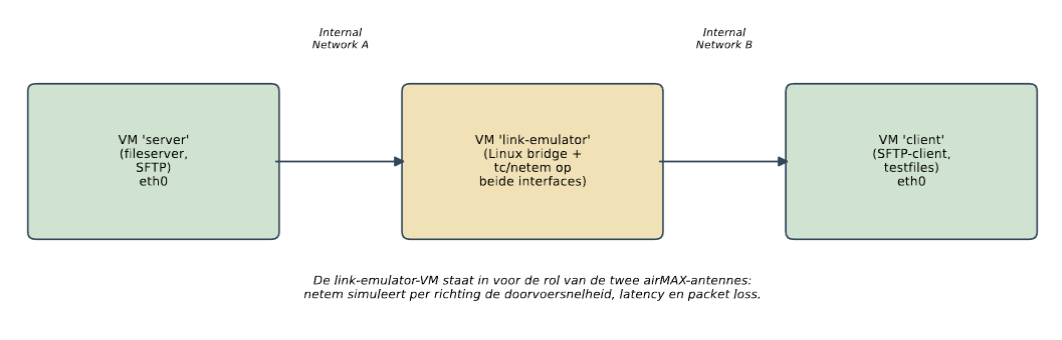
\includegraphics[width=\textwidth]{dumbbell_linkemulator.pdf}
  \caption{Dumbbell-topologie met een aparte link-emulator-VM die de twee airMAX-antennes vervangt. Enkel de link-emulator past \texttt{tc/netem} toe op de gebridgde interfaces.}
  \label{fig:dumbbell-linkemulator}
\end{figure}

De virtuele testopstelling bestaat uit drie geïsoleerde VirtualBox-VM's:
\begin{itemize}
  \item \textbf{VM 'poc-server':} Draait een Ubuntu Server-omgeving geconfigureerd als beveiligde SFTP-server (ondersteunt eisen FR1--FR3). De server is gekoppeld aan het virtuele netwerk \textit{Internal Network A}.
  \item \textbf{VM 'poc-link-emulator':} Een Linux-gebaseerde virtuele bridge geplaatst tussen \textit{Internal Network A} en \textit{Internal Network B}. Deze VM fungeert als transparante Layer-2 brug waarop onafhankelijk van de eindpunten Traffic Control (\texttt{tc}) en Network Emulation (\texttt{netem}) qdiscs worden toegepast.
  \item \textbf{VM 'poc-client':} Draait eveneens Ubuntu Server en bevat de geautomatiseerde SFTP-client, testscripts en meetinstrumentatie (\texttt{iperf3}, \texttt{mtr}, \texttt{tshark}). Deze VM is gekoppeld aan \textit{Internal Network B}.
\end{itemize}

Om beheer, uitrol en gegevensverzameling mogelijk te maken zonder het testverkeer te beïnvloeden, beschikt elke VM over een gescheiden beheerinterface (\texttt{nic1}) die via VirtualBox NAT gekoppeld is aan de host. SSH-poortforwarding op de host (poorten 2221, 2222 en 2223) biedt directe toegang tot respectievelijk de server, de link-emulator en de client.

\section{Geautomatiseerde Opbouw van de Testomgeving}%
\label{sec:automatisering-poc}

Om de reproduceerbaarheid van het onderzoek te garanderen (Sectie~\ref{sec:meth-verantwoording}), is de volledige configuratie en uitrol herleid tot één masterscript: \texttt{build\_poc.sh} (zie Bijlage~\ref{app:poc-scripts}). Het script maakt gebruik van het officiële Ubuntu 22.04 LTS Cloud Image (\texttt{qcow2}/\texttt{vmdk}) en provisioneert elke VM volledig onbewaakt via het \texttt{cloud-init} \textit{NoCloud}-databronmechanisme.

\subsection{Overzicht van het Buildscript}%
\label{subsec:automatisering-overzicht}

Het uitrolscript \texttt{build\_poc.sh} doorloopt opeenvolgend vijf geautomatiseerde fasen:
\begin{enumerate}
  \item \textbf{Image-preparatie:} Controleren van de aanwezigheid van het Ubuntu 22.04 Cloud-image en het converteren van het \texttt{.qcow2}-formaat naar een virtuele VirtualBox-schijf (\texttt{.vmdk}).
  \item \textbf{Opruimfase:} Bestaande VM-instanties en gekoppelde virtuele schijven gecontroleerd stoppen en verwijderen om een schone starttoestand te garanderen.
  \item \textbf{VM-provisionering:} Aanmaken van de drie VM's, aanpassen van de hardwareallocaties (CPU, RAM) en het genereren van specifieke \texttt{cloud-init} ISO-bestanden per rol.
  \item \textbf{Netwerkkoppeling:} Toewijzen van de interne VirtualBox-netwerken en NAT-portforwarding-regels via \texttt{VBoxManage}.
  \item \textbf{Validatie:} Wachten op SSH-beschikbaarheid via de beheersinterfaces en het weergeven van het netwerkoverzicht.
\end{enumerate}

Het onderstaande codefragment illustreert de centrale aanroep binnen \texttt{build\_poc.sh} waarmee de drie rollen parallel worden gedefinieerd:

\begin{lstlisting}[language=bash, caption={[Aanmaak van de drie PoC-VM's]Aanroep van de \texttt{create\_vm}-functie voor de drie roldefinities binnen het uitrolscript.}, label={lst:create-vm-calls}]
#!/usr/bin/env bash
# Aanmaak van de drie PoC-VM's via build_poc.sh
source ./config.sh

echo "[+] Bouwen van de PoC virtuele testomgeving..."

# Aanroepen van create_vm voor elke specifieke rol in de dumbbell-topologie
create_vm "poc-server"        "server"        "${SSH_PORT_SERVER}"  "${NET_LINK_A}"
create_vm "poc-link-emulator" "link-emulator" "${SSH_PORT_LINKEMU}" "${NET_LINK_A}" "${NET_LINK_B}"
create_vm "poc-client"        "client"        "${SSH_PORT_CLIENT}"  "${NET_LINK_B}"

echo "[+] Alle VM's zijn succesvol aangemaakt en gestart."
\end{lstlisting}

De herbruikbare functie \texttt{create\_vm} declareert de VM-parameters, initialiseert de opslagcontrollers en koppelt de virtuele schijven en ISO-bestanden aan de virtuele machine via de CLI-tool \texttt{VBoxManage}:

\begin{lstlisting}[language=bash, caption={[VBoxManage-aanroepen voor VM-aanmaak]Gedetailleerde implementatie van de \texttt{create\_vm}-functie.}, label={lst:vboxmanage-create}]
create_vm() {
    local vmname="$1"
    local role="$2"
    local mgmt_port="$3"
    local net_a="$4"
    local net_b="$5"

    echo "[*] Aanmaken van VM: ${vmname} (Rol: ${role})..."

    # 1. Registreer de VM in VirtualBox
    VBoxManage createvm --name "${vmname}" --ostype "Ubuntu_64" --register

    # 2. Configureer CPU, RAM, USB en Beheers-NAT-interface (NIC1)
    VBoxManage modifyvm "${vmname}" \
        --memory "${VM_MEMORY_MB}" \
        --cpus "${VM_CPUS}" \
        --nic1 nat \
        --natpf1 "ssh,tcp,127.0.0.1,${mgmt_port},,22" \
        --nic2 intnet --intnet2 "${net_a}" \
        --audio none --usb off

    # Optioneel: Voeg derde NIC toe voor de link-emulator (Layer-2 bridge)
    if [ -n "${net_b}" ]; then
        VBoxManage modifyvm "${vmname}" --nic3 intnet --intnet3 "${net_b}"
    fi

    # 3. Koppel de virtuele harde schijf en de seed.iso (cloud-init)
    VBoxManage storagectl "${vmname}" --name "SATA" --add sata --controller IntelAHCI
    VBoxManage storageattach "${vmname}" --storagectl "SATA" --port 0 \
        --device 0 --type hdd --medium "${VM_DIR}/${vmname}.vmdk"
    VBoxManage storageattach "${vmname}" --storagectl "SATA" --port 1 \
        --device 0 --type dvddrive --medium "${CONF_DIR}/${vmname}-seed.iso"

    # 4. Start de VM headless op
    VBoxManage startvm "${vmname}" --type headless
}
\end{lstlisting}

\subsection{Automatische Provisionering via cloud-init}%
\label{subsec:automatisering-cloudinit}

Om handmatige interactie met het besturingssysteem volledig uit te sluiten, worden de specifieke rol-instellingen gedefinieerd in \texttt{cloud-init}-manifesten (\texttt{user-data} en \texttt{meta-data}). Tijdens het eerste opstartproces leest het systeem deze instellingen uit van een virtuele cd-rom (\texttt{seed.iso}).

Op de server-VM richt \texttt{cloud-init} geautomatiseerd de netwerkinterface in, maakt een toegewijde SFTP-gebruikersaccount aan en configureert een \texttt{chroot}-omgeving binnen OpenSSH (ter ondersteuning van FR3, BR1 en BR2):

\begin{lstlisting}[language=yaml, caption={[Cloud-init: SFTP-chroot op de server-VM]Cloud-init manifest voor het inrichten van een beveiligde SFTP-chroot op de server-VM.}, label={lst:cloudinit-server-sftp}]
#cloud-config
hostname: poc-server
manage_etc_hosts: true

users:
  - name: sftpuser
    gecos: SFTP Test User
    lock_passwd: false
    plain_text_passwd: "sftp_password_poc"
    shell: /usr/sbin/nologin

write_files:
  - path: /etc/ssh/sshd_config.d/99-poc-sftp.conf
    owner: root:root
    permissions: '0644'
    content: |
      Match User sftpuser
          ChrootDirectory /srv/sftp
          ForceCommand internal-sftp
          AllowTcpForwarding no
          X11Forwarding no

runcmd:
  - mkdir -p /srv/sftp/uploads
  - chown root:root /srv/sftp
  - chmod 755 /srv/sftp
  - chown sftpuser:sftpuser /srv/sftp/uploads
  - systemctl restart ssh
\end{lstlisting}

Op de link-emulator-VM moet het verkeer tussen \textit{Internal Network A} en \textit{Internal Network B} op Layer~2 transparant doorgestuurd worden. Hiervoor declareert \texttt{cloud-init} een Netplan-configuratie die de fysieke interfaces \texttt{eth1} en \texttt{eth2} bundelt in een softwarematige netwerkbrug (\texttt{br0}):

\begin{lstlisting}[language=bash, caption={[Cloud-init: L2-brug op de link-emulator]Netplan-declaratie van de Layer-2 bridge op de link-emulator-VM.}, label={lst:cloudinit-bridge}]
#!/usr/bin/env bash
# Netplan bridge-configuratie gegenereerd op de link-emulator via cloud-init

cat << 'NETPLAN' > /etc/netplan/60-poc-bridge.yaml
network:
  version: 2
  renderer: networkd
  ethernets:
    eth0:
      dhcp4: true
    eth1:
      dhcp4: false
      dhcp6: false
    eth2:
      dhcp4: false
      dhcp6: false
  bridges:
    br0:
      interfaces: [eth1, eth2]
      dhcp4: false
      dhcp6: false
      addresses: [192.168.10.254/24]
NETPLAN

netplan apply
\end{lstlisting}

\section{Van Datasheet naar tc/netem Parameters}%
\label{sec:sim-parameters}

Om de virtuele bridge het gedrag van een fysieke straalverbinding te laten vertonen, worden de parameters voor de emulatie afgeleid uit de officiële specificaties van de Ubiquiti airMAX AC-productlijn~\autocite{AirMaxTDMA, UISPGPSSync}.

\begin{figure}[h]
  \centering
  \includegraphics[width=\textwidth]{airmax_scenarios.pdf}
  \caption{Overzicht van de drie gesimuleerde kanaalscenario's en hun fysieke weergave op de link-emulator.}
  \label{fig:airmax-scenarios}
\end{figure}

Op de bridge-interface \texttt{eth1} van de link-emulator worden met het Linux-rtt-subsysteem Traffic Control (\texttt{tc}) en de netwerkemulatormodule (\texttt{netem}) concrete qdiscs (queueing disciplines) ingesteld. Er zijn drie representatieve testscenario's gedefinieerd (zie Figuur~\ref{fig:airmax-scenarios}):

\paragraph{Scenario 1 -- Ideaal (0--15 km, sterke Line-of-Sight):}
Representeert een optimale PtP-verbinding met hoge signaal-ruisverhouding (SNR) en maximale modulatie (256QAM).
\begin{verbatim}
sudo tc qdisc add dev eth1 root netem delay 12ms 2ms distribution normal \
    loss 0.1% rate 150mbit
\end{verbatim}

\paragraph{Scenario 2 -- Marginaal (15--30 km, verminderde signaalkwaliteit):}
Simuleert een langere afstand of toenemende atmosferische demping (regenval, obstakels in de eersten Fresnel-zone). De modulatie valt terug naar QPSK/16QAM met een hogere bitfoutfrequentie (BER).
\begin{verbatim}
sudo tc qdisc add dev eth1 root netem delay 22ms 3ms distribution normal \
    loss 1.5% rate 35mbit
\end{verbatim}

\paragraph{Scenario 3 -- DFS-kanaalwissel (radardetectie en onderbreking):}
Simuleert het wettelijk verplichte gedrag bij Dynamic Frequency Selection (DFS) conform norm EN~301~893. Indien de antenne radarsignalen detecteert op de 5.6~GHz-band, treedt een verplichte \textit{Channel Move Time} op. Dit scenario induceert een totale uitval van 10 seconden, gevolgd door een herstel naar marginale verbindingswaarden, om het automatische herstelvermogen van SFTP-overdrachten (FR6) te valideren:
\begin{verbatim}
# Fase A: Initiateer 100% packet loss (totale lijnonderbreking)
sudo tc qdisc change dev eth1 root netem loss 100%

# Fase B: Wacht gedurende de gesimuleerde DFS-omschakeltijd
sleep 10

# Fase C: Herstel het kanaal naar marginale operationele parameters
sudo tc qdisc change dev eth1 root netem delay 22ms 3ms distribution normal \
    loss 1.5% rate 35mbit
\end{verbatim}

\section{Uitvoering en Testmethodiek}%
\label{sec:sim-uitvoering}

De uitvoering van de metingen is gestroomlijnd via de ondersteunende sturingsscripts \texttt{scenario-select.sh} en \texttt{run-tests.sh}. Hiermee wordt de meetreeks volledig autonoom en reproduceerbaar uitgevoerd vanaf het beheersstation.

\begin{lstlisting}[language=bash, caption={[Volledige test-workflow]De gestandaardiseerde workflow van uitrol, scenario-selectie en test-uitvoering.}, label={lst:workflow-volledig}]
#!/usr/bin/env bash
# Volledige uitvoerings-workflow voor het testen van het PoC

# 1. Bouw de omgeving op en start de drie VM's
cd poc-scripts/
./build_poc.sh

# 2. Selecteer het te evalueren kanaalscenario op de link-emulator
./scenario-select.sh marginaal

# 3. Voer de geautomatiseerde meetreeks uit vanaf de client-VM
./run-tests.sh --output-dir ../resultaten/marginaal/
\end{lstlisting}

De meetmethodiek op de client-VM gebruikt drie complementaire analysetools:
\begin{itemize}
  \item \texttt{iperf3}: Verzamelt gegevens over de ruwe TCP-doorvoersnelheid en netwerkverzadiging (toetst aan REQ-01).
  \item \texttt{mtr} / \texttt{ping}: Bepaalt de statistische verdeling van RTT (latency), variantie (jitter) en pakketverlies op de gebridgde link (toetst aan REQ-02).
  \item \texttt{sftp} in combinatie met \texttt{tshark}: Voert een gestandaardiseerde bestandsoverdracht uit (100~MB testbestand) en legt de TCP-pakketstroom vast. Hieruit worden de effectieve TCP-windowgrootte, heroverdrachten (\textit{retransmissions}) en de invloed van SSH-buffers geanalyseerd (toetst aan REQ-03).
\end{itemize}

De via dit proces gegenereerde logbestanden en PCAP-pakkettraces vormen de directe input voor de resultatenanalyse en kwaliteitsevaluatie in Hoofdstuk~\ref{ch:resultaten-en-evaluatie}.
%%=============================================================================
%% Hoofdstuk: Resultaten en Evaluatie
%%=============================================================================

\chapter{Resultaten en Evaluatie}%
\label{ch:resultaten-en-evaluatie}

Dit hoofdstuk presenteert en interpreteert de meetresultaten van de proof-of-concept uit
Hoofdstuk~\ref{ch:proof-of-concept}. Voor elk van de drie afstandscategorieën uit
Hoofdstuk~\ref{ch:requirementsanalyse} (0--15~km, 15--30~km en 30+~km) werden honderd
onafhankelijke trials uitgevoerd met \href{code/scripts/Run-DistanceTrials.ps1}{\texttt{Run-DistanceTrials.ps1}},
waarbij elke trial een eigen, willekeurige weers- en DFS-realisatie kreeg
(Sectie~\ref{sec:sim-parameters}). Dat levert in totaal 300 onafhankelijke metingen op,
waarmee de architectuur niet enkel op een enkel gunstig moment, maar over een
representatieve steekproef van mogelijke kanaalomstandigheden geëvalueerd kan worden.

\section{Methodologie van de metingen}%
\label{sec:res-methodologie}

Elke trial verliep volgens hetzelfde protocol: eerst kreeg de link-emulator via
\texttt{poc-run-trial.sh} een nieuwe, willekeurige combinatie van vertraging,
doorvoersnelheidsbeperking en Gilbert-Elliot-burstverlies opgelegd, gecentreerd rond de
basiswaarden van de gekozen afstandscategorie (Sectie~\ref{subsec:willekeurige-trial}).
Onafhankelijk daarvan kreeg elke trial een kans van 8\% op een bijkomende
DFS-onderbreking, ongeacht de afstandscategorie, zoals vereist. Vervolgens werd
gedurende een meetvenster van 30~seconden het effectieve packet loss tussen client en
server gemeten met \texttt{ping} (30 pakketten, 1 per seconde) -- een venster dat
ruimschoots volstaat om een eventuele DFS-onderbreking (uiterlijk na 18~seconden
volledig afgerond) mee op te vangen.

Deze batchmethodologie is specifiek gericht op REQ-03 (packet loss-tolerantie) en FR-06
(hervatten na onderbreking). De doorvoersnelheid (REQ-01) en de latency/jitter (REQ-02)
werden, zoals beschreven in Sectie~\ref{sec:sim-uitvoering}, afzonderlijk gevalideerd via
\texttt{Run-Tests.ps1} en vallen buiten de omvang van de 300 batchtrials in dit
hoofdstuk.

Om een zuiver antwoord te geven op de vraag of de architectuur onder \emph{normale}
kanaalomstandigheden aan REQ-03 voldoet, worden de resultaten per afstandscategorie
telkens in drie groepen opgesplitst: alle trials samen (het ruwe gemiddelde), enkel de
trials \emph{zonder} DFS-gebeurtenis (relevant voor REQ-03), en enkel de trials
\emph{met} een DFS-gebeurtenis (relevant voor FR-06). Deze opsplitsing werd berekend met
\href{code/scripts/Analyze-Trials.ps1}{\texttt{Analyze-Trials.ps1}} op basis van de
ruwe, per trial weggeschreven CSV-bestanden.

\section{Resultaten per afstandscategorie}%
\label{sec:res-resultaten}

Tabel~\ref{tab:resultaten-per-afstand} vat de statistische verdeling van het gemeten
packet loss samen voor elk van de drie afstandscategorieën, telkens opgesplitst volgens
Sectie~\ref{sec:res-methodologie}. Figuur~\ref{fig:packetloss_per_afstand} toont
dezelfde gegevens grafisch.

\begin{table}[h]
  \centering
  \small
  \begin{tabular}{p{2.0cm}p{2.6cm}p{1.3cm}p{1.9cm}p{1.9cm}p{1.7cm}p{1.9cm}}
    \toprule
    \textbf{Afstand} & \textbf{Groep} & \textbf{$n$} & \textbf{Gem.} & \textbf{Std.dev.} & \textbf{Min/Max} & \textbf{$>$REQ-03} \\
    \midrule
    0--15~km & Alle trials        & 100 & 2{,}43\%  & 8{,}31\%  & 0{,}00 / 36{,}67\% & 15/100 \\
    0--15~km & Zonder DFS         & 94  & 0{,}35\%  & 1{,}14\%  & 0{,}00 / 6{,}67\%  & 9/94   \\
    0--15~km & Met DFS            & 6   & 35{,}00\% & 1{,}67\%  & 33{,}33 / 36{,}67\% & 6/6   \\
    \midrule
    15--30~km & Alle trials        & 100 & 7{,}37\%  & 8{,}87\%  & 0{,}00 / 36{,}67\% & 78/100 \\
    15--30~km & Zonder DFS         & 93  & 5{,}27\%  & 4{,}65\%  & 0{,}00 / 20{,}00\% & 71/93  \\
    15--30~km & Met DFS            & 7   & 35{,}24\% & 1{,}65\%  & 33{,}33 / 36{,}67\% & 7/7    \\
    \midrule
    30+~km & Alle trials        & 100 & 21{,}47\% & 10{,}85\% & 0{,}00 / 53{,}33\% & 99/100 \\
    30+~km & Zonder DFS         & 96  & 20{,}38\% & 9{,}62\%  & 0{,}00 / 46{,}67\% & 95/96  \\
    30+~km & Met DFS            & 4   & 47{,}50\% & 3{,}63\%  & 43{,}33 / 53{,}33\% & 4/4    \\
    \bottomrule
  \end{tabular}
  \caption{Statistische verdeling van het gemeten packet loss per afstandscategorie
  (100 trials elk), opgesplitst naar de aan- of afwezigheid van een DFS-gebeurtenis
  tijdens de trial. "$>$REQ-03" geeft het aantal trials weer dat de norm van maximaal
  2\% packet loss overschrijdt.}
  \label{tab:resultaten-per-afstand}
\end{table}

\begin{figure}[h]
  \centering
  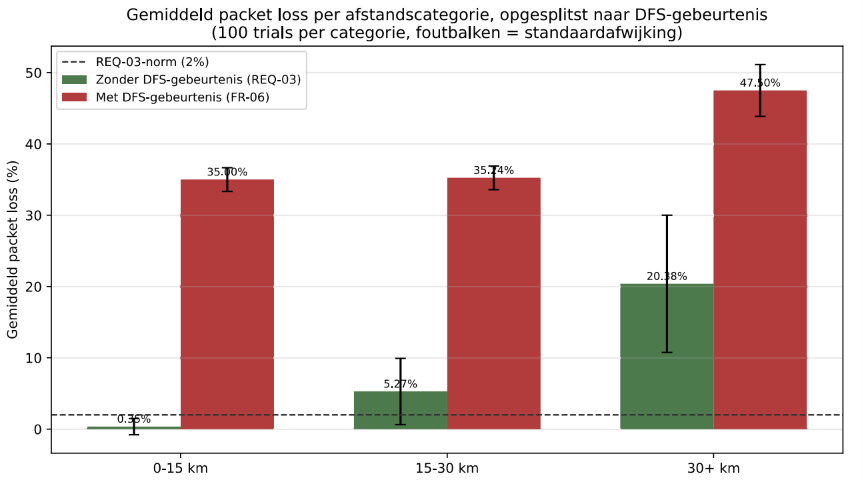
\includegraphics[width=\textwidth]{packetloss_per_afstand.png}
  \caption{Gemiddeld packet loss per afstandscategorie, opgesplitst naar trials zonder
  (groen, REQ-03) en met (rood, FR-06) DFS-gebeurtenis. De stippellijn markeert de
  REQ-03-norm van 2\%. Foutbalken tonen de standaardafwijking.}
  \label{fig:packetloss_per_afstand}
\end{figure}

\section{Interpretatie}%
\label{sec:res-interpretatie}

De drie afstandscategorieën vertonen een duidelijk, oplopend patroon dat niet toevallig
is, maar rechtstreeks voortvloeit uit de progressief zwaardere basisparameters die in
Sectie~\ref{sec:sim-parameters} per categorie werden vastgelegd. Toch verschilt de
\emph{oorzaak} van eventuele REQ-03-overschrijding sterk per categorie, wat enkel
zichtbaar wordt dankzij de DFS-opsplitsing.

\paragraph{0--15~km: REQ-03 wordt gehaald onder normale werking.} Zonder DFS-gebeurtenis
bedraagt het gemiddelde packet loss slechts 0{,}35\%, ruim onder de norm van 2\%. Van de
94 trials zonder DFS overschrijden er slechts 9 de norm, telkens met een beperkte
overschrijding (maximaal 6{,}67\%). De overige 6 trials met een REQ-03-overschrijding
gaan uitsluitend terug op een DFS-gebeurtenis: bij die trials ligt het verlies steevast
rond 33--37\%, een waarde die rechtstreeks te verklaren is uit een volledige
onderbreking van ongeveer 10~seconden binnen een meetvenster van 30~seconden
($10/30 \approx 33\%$). Voor deze afstandscategorie is REQ-03 dus een correcte
weerspiegeling van een goed presterend kanaal: de architectuur voldoet aan de eis onder
normale omstandigheden, en de enige uitzonderingen zijn een rechtstreeks, verwacht
gevolg van een verplichte regelgevende gebeurtenis (Sectie~\ref{subsec:dfs}) -- precies
het scenario waarvoor FR-06 bedoeld is, niet een tekortkoming van de link zelf.

\paragraph{15--30~km: REQ-03 wordt structureel overschreden, ook zonder DFS.} Hier
bedraagt het gemiddelde packet loss zonder DFS al 5{,}27\%, meer dan het dubbele van de
norm, en overschrijden 71 van de 93 niet-DFS-trials (76{,}3\%) de norm. In tegenstelling
tot de 0--15~km-categorie is de REQ-03-overschrijding hier dus \emph{niet} voornamelijk
een DFS-effect, maar een gevolg van de courante, alledaagse kanaalkwaliteit op deze
afstand. De DFS-trials (gemiddeld 35{,}24\%) volgen wel nog steeds hetzelfde patroon als
bij 0--15~km, wat aantoont dat het herstelgedrag na een onderbreking (FR-06) op deze
afstand identiek robuust blijft; het is de basiskwaliteit van de verbinding zelf die
tekortschiet.

\paragraph{30+~km: de architectuur voldoet niet aan REQ-03.} Zonder DFS bedraagt het
gemiddelde packet loss 20{,}38\%, en overschrijden 95 van de 96 niet-DFS-trials de norm.
Op deze afstand is de REQ-03-overschrijding niet langer een grensgeval, maar
vrijwel universeel. Dit bevestigt kwantitatief de kwalitatieve inschatting uit
Sectie~\ref{sec:req-tussentijdse-conclusie}, waar 30+~km reeds werd omschreven als
liggend buiten het betrouwbare toepassingsgebied voor permanente bestandstoegang.

\paragraph{FR-06 (herstel na DFS-onderbreking) wordt op elke afstand consistent
gevalideerd.} Opvallend is dat het gemiddelde verlies bij DFS-trials weliswaar toeneemt
met de afstand (35{,}00\% → 35{,}24\% → 47{,}50\%), maar dat het patroon -- een pak van
het meetvenster volledig onbereikbaar, gevolgd door herstel binnen dezelfde trial --
op alle drie de afstanden aanwezig blijft. Dit toont aan dat de architectuur
(SFTP over TCP, in combinatie met de netem-gebaseerde DFS-simulatie) consequent in staat
is om van een verplichte kanaalonderbreking te herstellen, onafhankelijk van de
onderliggende afstandscategorie.

\section{Toetsing aan de requirements}%
\label{sec:res-toetsing}

Tabel~\ref{tab:res-toetsing} vat de toetsing van de statistische batchresultaten aan de
relevante requirements uit Hoofdstuk~\ref{ch:requirementsanalyse} samen.

\begin{table}[h]
  \centering
  \small
  \begin{tabular}{p{1.6cm}p{9.0cm}p{2.4cm}}
    \toprule
    \textbf{Vereiste} & \textbf{Toetsing} & \textbf{Resultaat} \\
    \midrule
    REQ-03 (0--15~km) & Packet loss $\le 2\%$ onder normale werking & \textbf{Voldaan} (0{,}35\%) \\
    REQ-03 (15--30~km) & Packet loss $\le 2\%$ onder normale werking & \textbf{Niet voldaan} (5{,}27\%) \\
    REQ-03 (30+~km) & Packet loss $\le 2\%$ onder normale werking & \textbf{Niet voldaan} (20{,}38\%) \\
    FR-06 (alle afstanden) & Herstel van SFTP-overdracht na een DFS-onderbreking & \textbf{Voldaan} op alle drie de afstanden \\
    \bottomrule
  \end{tabular}
  \caption{Toetsing van de statistische batchresultaten aan REQ-03 en FR-06.}
  \label{tab:res-toetsing}
\end{table}

\section{Besluit van dit hoofdstuk}%
\label{sec:res-besluit}

De 300 onafhankelijke trials, verdeeld over drie afstandscategorieën en met telkens een
eigen willekeurige weers- en DFS-realisatie, leveren een statistisch onderbouwd en
consistent beeld op. Binnen het optimale bereik (0--15~km) presteert de architectuur
ruim binnen de gestelde norm voor packet loss, met REQ-03-overschrijdingen die vrijwel
uitsluitend het rechtstreekse en verwachte gevolg zijn van een verplichte
DFS-onderbreking. Vanaf de horizonlimiet (15--30~km) schiet de courante kanaalkwaliteit
zelf reeds structureel tekort, en voorbij het als onbetrouwbaar bestempelde bereik
(30+~km) is die tekortkoming vrijwel universeel. Onafhankelijk van de afstand toont de
architectuur zich wel steeds in staat om een SFTP-overdracht na een DFS-onderbreking te
hervatten (FR-06), wat de robuustheid van de gekozen combinatie van SFTP en de
TCP-transportlaag bevestigt.

Deze resultaten geven, in combinatie met de eerder afzonderlijk gevalideerde
doorvoersnelheid en latency (REQ-01, REQ-02, Sectie~\ref{sec:sim-uitvoering}), een
genuanceerd antwoord op de centrale onderzoeksvraag: de voorgestelde architectuur is
geschikt voor toegang tot een private fileserver binnen het optimale bereik, maar niet
zonder meer voor de verder gelegen afstandscategorieën. De implicaties hiervan voor de
onderzoeksvraag en de aanbevelingen voor vervolgonderzoek worden verder uitgewerkt in
Hoofdstuk~\ref{ch:conclusie}.
%%=============================================================================
%% Conclusie
%%=============================================================================

\chapter{Conclusie}%
\label{ch:conclusie}

% TODO: Trek een duidelijke conclusie, in de vorm van een antwoord op de
% onderzoeksvra(a)g(en). Wat was jouw bijdrage aan het onderzoeksdomein en
% hoe biedt dit meerwaarde aan het vakgebied/doelgroep? 
% Reflecteer kritisch over het resultaat. In Engelse teksten wordt deze sectie
% ``Discussion'' genoemd. Had je deze uitkomst verwacht? Zijn er zaken die nog
% niet duidelijk zijn?
% Heeft het onderzoek geleid tot nieuwe vragen die uitnodigen tot verder 
%onderzoek?

Dit hoofdstuk beantwoordt de centrale onderzoeksvraag en de deelvragen uit
Hoofdstuk~\ref{ch:inleiding}, op basis van de theoretische bevindingen uit
Hoofdstuk~\ref{ch:stand-van-zaken} en de empirische resultaten uit
Hoofdstuk~\ref{ch:resultaten-en-evaluatie}. Vervolgens wordt de bijdrage van dit
onderzoek aan het vakgebied toegelicht, gevolgd door een kritische reflectie op de
gehanteerde aanpak en een aanzet voor toekomstig onderzoek.
 
\section{Antwoord op de centrale onderzoeksvraag}%
\label{sec:conclusie-hoofdvraag}
 
De centrale onderzoeksvraag luidde: \textit{hoe kan een verbinding worden opgezet met
een eigen fileserver via een radioverbinding, en wat zijn de technische randvoorwaarden
en maximale afstandsbeperkingen voor een werkende implementatie?}
 
Het antwoord is genuanceerd, en net die nuance vormt de kern van de bijdrage van dit
onderzoek. Een architectuur die een private fileserver via SFTP over een
point-to-point-straalverbinding ontsluit, is technisch haalbaar en presteert binnen het
optimale bereik (0--15~km) ruimschoots binnen de vooropgestelde eisen: het gemiddelde
packet loss onder normale kanaalomstandigheden bedroeg er slechts 0{,}35\%, ruim onder
de norm van 2\% (REQ-03, Sectie~\ref{sec:res-interpretatie}). Vanaf de horizonlimiet
(15--30~km) schiet diezelfde kanaalkwaliteit echter reeds structureel tekort (gemiddeld
5{,}27\% verlies), en voorbij het bereik dat in de requirementsanalyse als onbetrouwbaar
werd bestempeld (30+~km) is die tekortkoming vrijwel universeel (20{,}38\%). De
"maximale afstandsbeperking" uit de onderzoeksvraag is dus geen enkel harde grenswaarde,
maar een geleidelijke, kwantitatief in kaart gebrachte overgang: de architectuur is
\emph{geschikt} binnen ongeveer 15~km, \emph{grensgeval} tot ongeveer 30~km, en
\emph{ongeschikt} daarbuiten voor permanente, betrouwbare bestandstoegang.
 
Eén element van de architectuur bleek daarbij opmerkelijk consistent, ongeacht de
afstand: het vermogen om een bestandsoverdracht te hervatten na een verplichte,
wettelijk voorgeschreven kanaalonderbreking door Dynamic Frequency Selection (FR-06,
Sectie~\ref{subsec:dfs}). Op alle drie de afstandscategorieën herstelde de combinatie
van SFTP en TCP zich betrouwbaar van zo'n onderbreking, wat aantoont dat deze
protocolkeuze een robuuste basis vormt, onafhankelijk van de onderliggende
kanaalkwaliteit.
 
\section{Antwoord op de deelvragen}%
\label{sec:conclusie-deelvragen}
 
\paragraph{Welke radioprotocollen zijn geschikt voor bestandsoverdracht?} De
literatuurstudie (Hoofdstuk~\ref{ch:stand-van-zaken}) toonde aan dat klassieke
amateurradioprotocollen zoals AX.25 en Winlink, hoewel robuust en breed inzetbaar voor
noodcommunicatie, primair ontworpen zijn voor tekstgebaseerde berichten met een lage
bandbreedte, en zich niet lenen tot het efficiënt overdragen van bestanden van
enige omvang. Native IP-over-radio -- het tunnelen van gewoon IP-verkeer over een
radioverbinding, waardoor bestaande, standaard bestandsoverdrachtsprotocollen hergebruikt
kunnen worden -- bleek de geschiktere aanpak. Binnen die protocollen is specifiek SFTP
gekozen boven bijvoorbeeld SMB, omwille van zijn beperkte "chattiness" (minder
gevoelig voor latency- en jitterschommelingen, Sectie~\ref{sec:req-tussentijdse-conclusie})
en zijn ingebouwde authenticatie en versleuteling.
 
\paragraph{Welke multiplextechnieken zijn van toepassing, en welke beperkingen leggen
zij op?} OFDM werd in de literatuurstudie geïdentificeerd als de meest geschikte
multiplextechniek voor instabiele radiokanalen, dankzij zijn robuustheid tegen
multipath-fading en looptijdverschillen (Sectie~\ref{sec:Multiplextechnieken in radiogebaseerde datacommunicatie}).
Deze keuze kon in de proof-of-concept echter niet rechtstreeks empirisch geverifieerd
worden: de gebruikte netwerkemulatie (Hoofdstuk~\ref{ch:proof-of-concept}) simuleert het
gedrag van de fysieke laag op basis van statistische parameters (vertraging,
doorvoersnelheid, burstverlies), maar bootst geen daadwerkelijke modulatie of
multiplexing na. Dit blijft dan ook een aanbeveling voor verder onderzoek
(Sectie~\ref{sec:conclusie-verder-onderzoek}).
 
\paragraph{Wat is de maximale praktische afstand?} Dit is de deelvraag waarop dit
onderzoek het meest concrete antwoord biedt, samengevat in
Sectie~\ref{sec:conclusie-hoofdvraag} hierboven en in detail onderbouwd in
Tabel~\ref{tab:resultaten-per-afstand} en Tabel~\ref{tab:res-toetsing}. In tegenstelling
tot een eenmalige meting op een enkele afstand, geeft de statistische onderbouwing over
300 trials (100 per afstandscategorie, met telkens een willekeurige weers- en
DFS-realisatie) een betrouwbaar beeld van de \emph{spreiding} van de haalbare prestaties,
niet enkel van een toevallig gunstig of ongunstig moment.
 
\paragraph{Welke minimale infrastructuur en configuratie zijn vereist?} Hoofdstuk~\ref{ch:proof-of-concept}
beschrijft de minimale opstelling in detail: een SFTP-server met een chroot-omgeving
voor de gebruiker, een netwerkbrug die de radioverbinding representeert, en een client
met standaard SFTP-, meet- en diagnosetools. De volledige opstelling -- van installatie
tot statistisch onderbouwde meting -- is bovendien volledig geautomatiseerd, wat het
antwoord op deze deelvraag ook onmiddellijk reproduceerbaar en overdraagbaar maakt naar
andere onderzoekers of praktijksituaties.
 
\section{Bijdrage aan het vakgebied en meerwaarde voor de doelgroep}%
\label{sec:conclusie-bijdrage}
 
De literatuurstudie in Hoofdstuk~\ref{ch:stand-van-zaken} identificeerde een lacune in
de bestaande vakliteratuur: onderzoek naar radiogebaseerde communicatie richt zich
overwegend op noodcommunicatie, professionele draadloze backhaul, of berichtenverkeer,
maar niet specifiek op de toegankelijkheid van een persoonlijke of kleinschalige
fileserver. Dit onderzoek vult die lacune op met een kwantitatief, per afstand
gedifferentieerd antwoord, dat rechtstreeks bruikbaar is voor de in
Sectie~\ref{sec:probleemstelling} geïdentificeerde doelgroep: maritieme operatoren,
hulpverleningsorganisaties, onderzoekers in afgelegen gebieden en radioamateurs kunnen
uit dit onderzoek een concreet, onderbouwd beeld meenemen van tot welke afstand een
dergelijke opstelling betrouwbaar inzetbaar is, en welke architecturale keuzes (SFTP,
DFS-conforme apparatuur) daarbij aangewezen zijn.
 
Daarnaast levert dit onderzoek een methodologische bijdrage die verder reikt dan de
specifieke onderzoeksvraag: de volledig geautomatiseerde, statistisch onderbouwde
testmethodologie uit Hoofdstuk~\ref{ch:proof-of-concept} -- met een Gilbert-Elliot-
burstverliesmodel voor weersvariatie en een stochastische DFS-simulatie, herhaald over
honderden onafhankelijke trials -- is generiek genoeg om ook voor andere
radiogebaseerde of draadloze netwerkonderzoeken te worden hergebruikt. Waar veel
kleinschalige proof-of-concept-onderzoeken zich beperken tot een handvol
puntmetingen, toont dit onderzoek aan dat een statistisch representatieve steekproef,
ook binnen de tijdspanne van een bachelorproef, haalbaar en waardevol is.
 
\section{Kritische reflectie}%
\label{sec:conclusie-reflectie}
 
Het algemene patroon van afnemende kanaalkwaliteit met toenemende afstand was verwacht:
zowel de wet van Shannon-Hartley (Hoofdstuk~\ref{ch:stand-van-zaken}) als de
kwalitatieve inschatting in de requirementsanalyse (Sectie~\ref{sec:req-tussentijdse-conclusie})
voorspelden dat de 30+~km-categorie buiten het betrouwbare toepassingsgebied zou vallen.
De mate waarin dit vermoeden nu kwantitatief bevestigd wordt -- 99\% van de trials
overschrijdt er de norm, tegenover slechts 15\% bij 0--15~km -- was echter scherper dan
op voorhand kon worden aangenomen. Minder verwacht was het onderscheid dat de
DFS-opsplitsing binnen de 15--30~km-categorie blootlegde: daar bleek de
REQ-03-overschrijding \emph{niet} voornamelijk het gevolg van de verplichte
DFS-onderbrekingen (zoals bij 0--15~km), maar van de courante kanaalkwaliteit zelf. Dat
onderscheid was pas zichtbaar dankzij de expliciete opsplitsing van de resultaten, en
onderstreept het belang van een voldoende gedetailleerde statistische analyse boven een
enkel, samengevat gemiddelde.
 
De belangrijkste beperking van dit onderzoek is methodologisch van aard, en werd reeds
uitgebreid toegelicht in Sectie~\ref{subsec:meth-bijstelling-fase3}: de voorziene
fysieke 5.6~GHz airMAX-straalverbinding kon niet worden aangekocht, waardoor de volledige
proof-of-concept via netwerkemulatie gerealiseerd werd. De gerapporteerde resultaten
tonen daardoor aan of de gekozen architectuur functioneel en performant is onder
\emph{verwachte}, uit officiële specificaties afgeleide kanaalcondities, maar
bevestigen niet de effectieve RF-prestaties -- antennealignment, werkelijke
signaalpropagatie, concrete weersinvloed -- van een fysieke link in het veld. De
gebruikte Gilbert-Elliot-parameters en DFS-kans zijn plausibele, uit de literatuur en
productspecificaties afgeleide schattingen, geen gemeten grootheden. Deze beperking
raakt met name de deelvraag over multiplextechnieken (Sectie~\ref{sec:conclusie-deelvragen}),
die in deze opstelling niet op fysiek niveau getoetst kon worden.
 
Een tweede, kleinere kanttekening betreft de asymmetrie in meetintensiteit tussen de
requirements: REQ-03 (packet loss) en FR-06 (DFS-herstel) werden dankzij hun
niet-deterministische aard over 300 trials statistisch onderbouwd, terwijl REQ-01
(doorvoersnelheid) en REQ-02 (latency/jitter) via een beperkter aantal metingen per
afstandscategorie werden gevalideerd (Sectie~\ref{sec:sim-uitvoering}). Een even
uitgebreide statistische onderbouwing van die laatste twee eisen zou het totaalbeeld
verder versterken.
 
\section{Aanbevelingen voor toekomstig onderzoek}%
\label{sec:conclusie-verder-onderzoek}
 
Op basis van de bevindingen en beperkingen hierboven worden de volgende richtingen voor
vervolgonderzoek voorgesteld:
 
\begin{itemize}
  \item \textbf{Fysieke veldvalidatie.} Zodra geschikte 5.6~GHz airMAX-apparatuur (of een
        vergelijkbaar alternatief) beschikbaar is, zou een fysieke herhaling van de
        drie afstandscategorieën toelaten om de in dit onderzoek gebruikte
        Gilbert-Elliot- en DFS-parameters te kalibreren aan werkelijke veldmetingen, en
        om architecturale aspecten (antennealignment, effectieve modulatie) te
        valideren die in een netwerkemulatie noodgedwongen buiten beschouwing bleven.
  \item \textbf{Uitbreiding van de statistische onderbouwing naar REQ-01 en REQ-02.} Een
        vergelijkbare batchmethodologie als voor packet loss (Hoofdstuk~\ref{ch:proof-of-concept})
        zou ook voor doorvoersnelheid en latency toegepast kunnen worden, voor een
        even robuust onderbouwd beeld van alle vier de netwerktechnische requirements.
  \item \textbf{Alternatieve frequentiebanden en vermogensklassen.} Dit onderzoek
        beperkte zich, om regelgevende redenen, tot de licentievrije 5.6~GHz-limieten
        (1~W EIRP). Een vergelijkende studie met het gelicentieerde amateursegment
        (tot 200~W PEP, Sectie~\ref{sec:req-tussentijdse-conclusie}) of met de 6m-band
        uit Hoofdstuk~\ref{ch:stand-van-zaken} zou kunnen uitwijzen of een groter bereik
        haalbaar is binnen een andere regelgevende context.
  \item \textbf{Multi-hop-oplossingen voor het onbetrouwbare bereik.} Voor de
        30+~km-categorie, waar dit onderzoek aantoonde dat een directe verbinding niet
        volstaat, zou onderzocht kunnen worden of een keten van meerdere, kortere
        straalverbindingen (relais) een uitkomst biedt -- elke afzonderlijke schakel
        zou dan binnen het in dit onderzoek als betrouwbaar aangetoonde bereik van
        0--15~km kunnen blijven.
  \item \textbf{Reële, gemeten weersdata.} In plaats van willekeurig getrokken
        Gilbert-Elliot-parameters binnen een plausibele bandbreedte, zou toekomstig
        onderzoek de simulatie kunnen voeden met effectief gemeten meteorologische
        gegevens (regenintensiteit, luchtvochtigheid) gekoppeld aan gelijktijdige
        signaalmetingen, voor een nog realistischer verband tussen weer en
        kanaalkwaliteit.
\end{itemize}
 
Samengevat toont dit onderzoek aan dat radiogebaseerde toegang tot een private
fileserver, binnen een zorgvuldig afgebakend afstandsbereik, een technisch haalbaar en
statistisch onderbouwd alternatief vormt voor de doelgroep uit
Sectie~\ref{sec:probleemstelling} -- met een duidelijk, kwantitatief in kaart gebracht
omslagpunt waarop toekomstig onderzoek verder kan bouwen.



%---------- Bijlagen -----------------------------------------------------------

\appendix

\chapter{Onderzoeksvoorstel}

Het onderwerp van deze bachelorproef is gebaseerd op een onderzoeksvoorstel dat vooraf werd beoordeeld door de promotor. Dat voorstel is opgenomen in deze bijlage.

%% TODO: 
%\section*{Samenvatting}

% Kopieer en plak hier de samenvatting (abstract) van je onderzoeksvoorstel.

% Verwijzing naar het bestand met de inhoud van het onderzoeksvoorstel
%---------- Inleiding ---------------------------------------------------------

% TODO: Is dit voorstel gebaseerd op een paper van Research Methods die je
% vorig jaar hebt ingediend? Heb je daarbij eventueel samengewerkt met een
% andere student?
% Zo ja, haal dan de tekst hieronder uit commentaar en pas aan.

%\paragraph{Opmerking}

% Dit voorstel is gebaseerd op het onderzoeksvoorstel dat werd geschreven in het
% kader van het vak Research Methods dat ik (vorig/dit) academiejaar heb
% uitgewerkt (met medesturent VOORNAAM NAAM als mede-auteur).
% 

\section{Inleiding}%
\label{sec:inleiding}

%Waarover zal je bachelorproef gaan? Introduceer het thema en zorg dat volgende zaken zeker duidelijk aanwezig zijn:

%\begin{itemize}
%  \item kaderen thema
%  \item de doelgroep
%  \item de probleemstelling en (centrale) onderzoeksvraag
%  \item de onderzoeksdoelstelling
%\end{itemize}

%Denk er aan: een typische bachelorproef is \textit{toegepast onderzoek}, wat betekent dat je start vanuit een concrete probleemsituatie in bedrijfscontext, een \textbf{casus}. Het is belangrijk om je onderwerp goed af te bakenen: je gaat voor die \textit{ene specifieke probleemsituatie} op zoek naar een goede oplossing, op basis van de huidige kennis in het vakgebied.

%De doelgroep moet ook concreet en duidelijk zijn, dus geen algemene of vaag gedefinieerde groepen zoals \emph{bedrijven}, \emph{developers}, \emph{Vlamingen}, enz. Je richt je in elk geval op it-professionals, een bachelorproef is geen populariserende tekst. Eén specifiek bedrijf (die te maken hebben met een concrete probleemsituatie) is dus beter dan \emph{bedrijven} in het algemeen.

%Formuleer duidelijk de onderzoeksvraag! De begeleiders lezen nog steeds te veel voorstellen waarin we geen onderzoeksvraag terugvinden.

%Schrijf ook iets over de doelstelling. Wat zie je als het concrete eindresultaat van je onderzoek, naast de uitgeschreven scriptie? Is het een proof-of-concept, een rapport met aanbevelingen, \ldots Met welk eindresultaat kan je je bachelorproef als een succes beschouwen?

In de hedendaagse digitale wereld spelen digitale bestanden een grote rol, zowel in privé- als in bedrijfscontext \autocite{MaritimeSurvey2022}. Documenten, onderzoeksgegevens en administratieve dossiers worden digitaal opgemaakt, bijgehouden en wereldwijd verspreid. Papieren documenten en boeken worden gedigitaliseerd om ze eenvoudig te verspreiden en te raadplegen. Hoewel dit het voor particulieren en bedrijven gemakkelijker maakt om een eigen bibliotheek aan informatie bij te houden, brengt dit ook complicaties met zich mee.

De grootste hiervan is toegankelijkheid. Wat gebeurt er wanneer men zich in een gebied bevindt zonder betrouwbare verbinding met het globale netwerk? Wat gebeurt er tijdens rampen, wanneer de infrastructuur wordt weggevaagd door tsunamis of aardbevingen \autocite{WinlinkEmcomm}? Wat zijn de beperkingen op zee, waar connectiviteit structureel onbetrouwbaar is \autocite{MaritimeSurvey2022}?

Hoewel er reeds oplossingen bestaan zoals Starlink en OneWeb, zijn deze voor particulieren en kleine bedrijven vaak financieel of praktisch ontoereikend. De alternatieven voor deze doelgroep zijn onvoldoende onderzocht. Bestaande draadloze communicatietechnologieën, zoals radioverbindingen, bieden potentieel een haalbaar alternatief, maar de toepasbaarheid ervan voor bestandsoverdracht op afstand is nog niet grondig in kaart gebracht.

\subsection*{Probleemstelling}

De centrale onderzoeksvraag luidt:

\begin{quote}
  \textit{Hoe kan een verbinding worden opgezet met een eigen fileserver via een radioverbinding, en wat zijn de technische randvoorwaarden en maximale afstandsbeperkingen voor een werkende implementatie?}
\end{quote}

Bijkomende deelvragen die het onderzoek structureren, zijn:

\begin{itemize}
  \item Welke radioprotocollen (zoals AX.25, Winlink, of IP-over-radio) zijn geschikt voor bestandsoverdracht, en wat zijn hun kenmerken op het vlak van bandbreedte, betrouwbaarheid en bereik?
  \item Welke multiplexingtechnieken — zoals \textit{frequency division multiplexing} (FDM) en \textit{time division multiplexing} (TDM) — zijn van toepassing binnen radiogebaseerde datacommunicatie, en welke beperkingen leggen zij op?
  \item Wat is de maximale praktische afstand waarover een bestandsoverdracht via radioverbinding haalbaar is, afhankelijk van frequentieband en omgevingsfactoren?
  \item Welke infrastructuur en configuratie zijn minimaal vereist voor een werkend proof-of-concept?
\end{itemize}

\subsection*{Doelgroep}

Dit onderzoek richt zich op IT-professionals en netwerkingenieurs die actief zijn in omgevingen met beperkte of onbetrouwbare internetconnectiviteit — zoals maritieme operatoren, hulpverleningsorganisaties in rampgebieden, of bedrijven in afgelegen regio's. De inzichten zijn tevens relevant voor radiocommunicatiespecialisten die netwerktoepassingen willen integreren in bestaande radioinfrastructuur.

\subsection*{Onderzoeksdoelstelling en methodologie}

Het doel van dit onderzoek is na te gaan of en hoe een fileserver bereikbaar gemaakt kan worden via een radioverbinding, met aandacht voor de technische haalbaarheid, de vereiste protocollen en de praktische beperkingen zoals maximale afstand en doorvoersnelheid.

De gehanteerde onderzoeksmethode omvat drie fasen:

\begin{enumerate}
  \item \textbf{Literatuurstudie:} Een grondige verkenning van relevante radioprotocollen (AX.25, Winlink, IP-over-radio), netwerktopologieën voor draadloze communicatie, en multiplexingtechnieken (FDM, TDM). Tevens worden de fysische eigenschappen van radiogolven bestudeerd, waaronder de invloed van frequentieband op bereik en datadoorvoer \autocite{Tanenbaum2021}.
  \item \textbf{Vergelijkende analyse:} De geïdentificeerde protocollen en technieken worden vergeleken op criteria zoals maximale afstand, bandbreedte, hardwarevereisten en complexiteit van implementatie.
  \item \textbf{Proof-of-concept:} Op basis van de analyse wordt een minimale werkende opstelling gebouwd en getest, bestaande uit een radiozender/-ontvanger en een fileserver, om de theoretische bevindingen empirisch te valideren.
\end{enumerate}

Het onderzoek kan drie mogelijke uitkomsten opleveren:

\begin{itemize}
  \item Een werkend proof-of-concept dat aantoont hoe een fileserver via radioverbinding bereikbaar gemaakt kan worden.
  \item Een theoretisch onderbouwde oplossingsarchitectuur die de implementatie mogelijk maakt, indien een volledig werkende opstelling buiten bereik valt.
  \item De gemotiveerde uitsluiting van radioverbindingen als haalbare oplossing voor dit probleem, op basis van vastgestelde technische beperkingen.
\end{itemize}

Naast het beantwoorden van de onderzoeksvraag beoogt dit onderzoek een basis te vormen voor verdere technologische ontwikkelingen en vervolgonderzoek binnen het domein van radiogebaseerde datacommunicatie.
%---------- Stand van zaken ---------------------------------------------------

\section{Literatuurstudie}%
\label{sec:literatuurstudie}

% Hier beschrijf je de \emph{state-of-the-art} rondom je gekozen onderzoeksdomein, d.w.z.\ een inleidende, doorlopende tekst over het onderzoeksdomein van je bachelorproef. Je steunt daarbij heel sterk op de professionele \emph{vakliteratuur}, en niet zozeer op populariserende teksten voor een breed publiek. Wat is de huidige stand van zaken in dit domein, en wat zijn nog eventuele open vragen (die misschien de aanleiding waren tot je onderzoeksvraag!)?

% Je mag de titel van deze sectie ook aanpassen (literatuurstudie, stand van zaken, enz.). Zijn er al gelijkaardige onderzoeken gevoerd? Wat concluderen ze? Wat is het verschil met jouw onderzoek?

% Verwijs bij elke introductie van een term of bewering over het domein naar de vakliteratuur, bijvoorbeeld~\autocite{Hykes2013}! Denk zeker goed na welke werken je refereert en waarom.

% Draag zorg voor correcte literatuurverwijzingen! Een bronvermelding hoort thuis \emph{binnen} de zin waar je je op die bron baseert, dus niet er buiten! Maak meteen een verwijzing als je gebruik maakt van een bron. Doe dit dus \emph{niet} aan het einde van een lange paragraaf. Baseer nooit teveel aansluitende tekst op eenzelfde bron.

% Als je informatie over bronnen verzamelt in JabRef, zorg er dan voor dat alle nodige info aanwezig is om de bron terug te vinden (zoals uitvoerig besproken in de lessen Research Methods).

% Voor literatuurverwijzingen zijn er twee belangrijke commando's:
% \autocite{KEY} => (Auteur, jaartal) Gebruik dit als de naam van de auteur
%   geen onderdeel is van de zin.
% \textcite{KEY} => Auteur (jaartal)  Gebruik dit als de auteursnaam wel een
%   functie heeft in de zin (bv. ``Uit onderzoek door Doll & Hill (1954) bleek
%   ...'')

% Je mag deze sectie nog verder onderverdelen in subsecties als dit de structuur van de tekst kan verduidelijken.

In deze literatuurstudie wordt de huidige stand van zaken binnen radiogebaseerde communicatie onderzocht, met nadruk op mogelijke oplossingen voor het zenden en ontvangen van digitale bestanden. Het doel is een conceptueel kader te schetsen dat als theoretische onderbouwing dient voor dit onderzoek.

\subsection{Connectiviteit in afgelegen gebieden en noodsituaties}

Toegang tot digitale bestanden is in de hedendaagse samenleving essentieel \autocite{MaritimeSurvey2022}, maar blijft in uiteenlopende situaties een uitdaging. Satellietnetwerken zoals Starlink en OneWeb bieden weliswaar globale dekking, maar kampen met hoge abonnementskosten, aanzienlijke latency en beperkte toegankelijkheid voor particulieren en kleine bedrijven \autocite{MaritimeSurvey2022}. In noodsituaties waarbij de bestaande infrastructuur is uitgevallen, blijft robuuste digitale communicatie bovendien een kritieke behoefte \autocite{WinlinkEmcomm}.

Deze beperkingen tonen aan dat er behoefte is aan alternatieve methoden die onafhankelijk zijn van een centrale infrastructuur, maar toch voldoende capaciteit kunnen garanderen voor het raadplegen van digitale bestanden.

\subsection{Radiofrequenties en signaalpropagatie}

Radiogebaseerde communicatie maakt gebruik van elektromagnetische golven die zich door de lucht voortplanten. De keuze van frequentieband heeft een directe invloed op zowel het maximale bereik als de beschikbare bandbreedte \autocite{Tanenbaum2021}. Lagere frequenties, zoals HF-banden (3--30 MHz), kunnen grote afstanden overbruggen via reflecties op de ionosfeer, maar bieden slechts een beperkte doorvoersnelheid. Hogere frequenties, zoals de VHF- (30--300 MHz) en UHF-banden (300 MHz--3 GHz), laten hogere datasnelheden toe, maar hebben een kleiner bereik en vereisen doorgaans een vrije zichtlijn tussen zender en ontvanger \autocite{Tanenbaum2021}.

De maximale praktische afstand van een radioverbinding wordt bepaald door een combinatie van factoren: zendvermogen, antenneversterking, frequentieband, terreinprofiel en atmosferische omstandigheden. Voor microwave point-to-point verbindingen in de GHz-range geldt een typisch operationeel bereik van enkele tientallen kilometers, mits er sprake is van \textit{line of sight} \autocite{MicrowavePtP5G}.

\subsection{Multiplextechnieken in radiogebaseerde datacommunicatie}

Om meerdere signalen efficiënt over een gedeeld radiokanaal te transporteren, worden multiplextechnieken toegepast \autocite{Tanenbaum2021}. De twee meest voorkomende zijn:

\begin{itemize}
  \item \textbf{Frequency Division Multiplexing (FDM):} Het beschikbare frequentiespectrum wordt opgedeeld in meerdere subbanden, elk toegewezen aan een afzonderlijk kanaal. Signalen worden gelijktijdig verzonden zonder elkaar te storen, op voorwaarde dat de subbanden voldoende van elkaar gescheiden zijn. FDM wordt veel gebruikt in analoge en digitale radiosystemen, waaronder FM-radio en 4G/LTE \autocite{Tanenbaum2021}.
  \item \textbf{Time Division Multiplexing (TDM):} Meerdere signalen maken gebruik van hetzelfde frequentiekanaal, maar worden afwisselend verzonden in vaste tijdsloten. TDM vereist nauwkeurige tijdssynchronisatie tussen zender en ontvanger, maar laat een efficiënter gebruik van de beschikbare bandbreedte toe wanneer niet alle kanalen continu actief zijn \autocite{Tanenbaum2021}.
\end{itemize}

In de praktijk worden deze technieken gecombineerd: moderne systemen zoals OFDM (\textit{Orthogonal Frequency Division Multiplexing}) integreren elementen van beide benaderingen en vormen de basis van hedendaagse draadloze standaarden \autocite{Tanenbaum2021}.

\subsection{Protocollen voor radiogebaseerde dataoverdracht}

Binnen de amateurradio-gemeenschap bestaan reeds systemen voor dataoverdracht via radiogolven. Een veelgebruikt protocol op de datalinklaag is AX.25, een pakketradioprotocol dat is afgeleid van het X.25-standaard en specifiek is ontworpen voor amateurradiocommunicatie \autocite{Tanenbaum2021}. AX.25 biedt foutdetectie en beperkte foutcorrectie, maar kent een lage doorvoersnelheid die het minder geschikt maakt voor grote bestandsoverdrachten.

Bovenop dergelijke protocollen zijn bredere systemen gebouwd, waarvan Winlink het meest gekende voorbeeld is. Winlink is een wereldwijd netwerk dat gebruikmaakt van HF-, VHF- en UHF-radiofrequenties om e-mailcommunicatie mogelijk te maken \autocite{WinlinkOverview}. Het wordt beschreven als een hybride radiosysteem, ontworpen voor communicatie in afgelegen gebieden en in noodsituaties \autocite{WinlinkEmcomm, WinlinkHybrid}. Hoewel Winlink beperkte bijlagen ondersteunt, is het primair ontworpen voor berichtuitwisseling en daarmee ontoereikend als volwaardige oplossing voor toegang tot een fileserver.

Een verdere optie is IP-over-radio: het tunnelen van standaard IP-verkeer over een radioverbinding, waardoor bestaande netwerktoepassingen — waaronder bestandsoverdrachten via protocollen zoals FTP of SMB — in principe over een radiokanaal kunnen worden aangeboden \autocite{Tanenbaum2021}. Dit concept vormt de theoretische basis voor de in dit onderzoek voorgestelde opstelling.

\subsection{Straalverbindingen als proof-of-concept}

Voor dit onderzoek wordt gefocust op straalverbindingen (\textit{point-to-point wireless links}), waarbij twee antennes rechtstreeks op elkaar gericht zijn. Deze opstelling biedt een grotere bandbreedte dan ionosferische propagatie \autocite{WirelessBackhaulSurvey, MicrowavePtP5G}, maar vereist een vrije zichtlijn (\textit{line of sight}) tussen beide antennes \autocite{MicrowavePtP5G}. In de praktijk worden dergelijke verbindingen al op grote schaal ingezet als draadloze backhaul in telecomnetwerken \autocite{WirelessBackhaulSurvey}.

De keuze voor een straalverbinding als proof-of-concept is verantwoord omdat dezelfde technologie en protocollen worden gebruikt als in grootschalige toepassingen, waardoor de resultaten overdraagbaar zijn naar bredere implementaties \autocite{WirelessBackhaulSurvey}.

\subsection{Lacunes in de bestaande kennis}

Hoewel diverse technologieën bestaan voor radiogebaseerde communicatie \autocite{MaritimeSurvey2022}, bespreekt geen van de onderzochte bronnen het gebruik ervan om toegang te bieden tot een persoonlijke fileserver. De bestaande literatuur richt zich voornamelijk op noodcommunicatie \autocite{WinlinkEmcomm}, professionele backhaul \autocite{MicrowavePtP5G, WirelessBackhaulSurvey} of beperkte diensten zoals e-mail \autocite{WinlinkOverview}. Dit onderzoek richt zich op de ontbrekende verbinding tussen deze deeldomeinen: de technische haalbaarheid van persoonlijke bestandstoegang via een zelfopgezette radioverbinding.

%---------- Methodologie ------------------------------------------------------
\section{Methodologie}%
\label{sec:methodologie}

%Hier beschrijf je hoe je van plan bent het onderzoek te voeren. Welke onderzoekstechniek ga je toepassen om elk van je onderzoeksvragen te beantwoorden? Gebruik je hiervoor literatuurstudie, interviews met belanghebbenden (bv.~voor requirements-analyse), experimenten, simulaties, vergelijkende studie, risico-analyse, PoC, \ldots?

%Valt je onderwerp onder één van de typische soorten bachelorproeven die besproken zijn in de lessen Research Methods (bv.\ vergelijkende studie of risico-analyse)? Zorg er dan ook voor dat we duidelijk de verschillende stappen terug vinden die we verwachten in dit soort onderzoek!

%Vermijd onderzoekstechnieken die geen objectieve, meetbare resultaten kunnen opleveren. Enquêtes, bijvoorbeeld, zijn voor een bachelorproef informatica meestal \textbf{niet geschikt}. De antwoorden zijn eerder meningen dan feiten en in de praktijk blijkt het ook bijzonder moeilijk om voldoende respondenten te vinden. Studenten die een enquête willen voeren, hebben meestal ook geen goede definitie van de populatie, waardoor ook niet kan aangetoond worden dat eventuele resultaten representatief zijn.

%Uit dit onderdeel moet duidelijk naar voor komen dat je bachelorproef ook technisch voldoen\-de diepgang zal bevatten. Het zou niet kloppen als een bachelorproef informatica ook door bv.\ een student marketing zou kunnen uitgevoerd worden.

%Je beschrijft ook al welke tools (hardware, software, diensten, \ldots) je denkt hiervoor te gebruiken of te ontwikkelen.

%Probeer ook een tijdschatting te maken. Hoe lang zal je met elke fase van je onderzoek bezig zijn en wat zijn de concrete \emph{deliverables} in elke fase?

Dit onderzoek hanteert een experimenteel-technische aanpak om te bepalen of een betrouwbare verbinding met een eigen fileserver via een radioverbinding haalbaar is. Het onderzoek is opgebouwd uit vier opeenvolgende fasen, elk met concrete deliverables en een geschatte doorlooptijd.

\subsection{Fase 1: Literatuurstudie}

In de eerste fase wordt de vakliteratuur rond radiogebaseerde dataoverdracht, straalverbindingen en fileserverprotocollen systematisch in kaart gebracht. Concreet komen de volgende onderwerpen aan bod:

\begin{itemize}
  \item Eigenschappen en beperkingen van radiofrequentiebanden (HF, VHF, UHF, microwave) met betrekking tot bandbreedte en maximaal bereik.
  \item Dataprotocollen voor radioverbindingen: AX.25, IP-over-radio en Winlink.
  \item Multiplextechnieken (FDM, TDM) en hun impact op doorvoersnelheid en kanaalbezetting.
  \item Wettelijke beperkingen voor radioamateurbanden in België (BIPT-regelgeving).
  \item Bestandsoverdrachtsprotocollen (FTP, SMB, SCP) en hun vereisten op netwerkniveau.
\end{itemize}

\textbf{Deliverable:} Een uitgewerkte literatuurstudie met een theoretisch kader en een overzicht van technische randvoorwaarden.

\subsection{Fase 2: Requirementsanalyse}

Op basis van de literatuurstudie worden meetbare functionele en niet-functionele eisen opgesteld waaraan de proefopstelling moet voldoen. Deze requirements omvatten onder meer:

\begin{itemize}
  \item \textbf{Minimale bandbreedte:} voldoende doorvoersnelheid voor het ophalen van bestanden binnen een aanvaardbare tijdsspanne.
  \item \textbf{Maximale latency:} de verbindingsvertraging mag de werking van het gekozen bestandsoverdrachtsprotocol niet verstoren.
  \item \textbf{Verbindingsstabiliteit:} maximaal aanvaardbaar packet loss percentage tijdens een overdracht.
  \item \textbf{Wettelijke conformiteit:} de gebruikte frequenties en zendvermogens voldoen aan de Belgische radioamateurregelgeving.
  \item \textbf{Maximale afstand:} de beoogde afstand tussen zender en ontvanger, bepaald op basis van de gekozen frequentieband en antenneconfiguratie.
\end{itemize}

\textbf{Deliverable:} Een gestructureerd requirements-document dat als toetsingskader dient voor de evaluatie van de proof-of-concept.

\subsection{Fase 3: Proof-of-Concept}

In de derde fase wordt een minimale werkende opstelling gebouwd en getest. De hardware bestaat uit twee computers — één geconfigureerd als fileserver, één als client — verbonden via een punt-tot-punt straalantenne-opstelling. De volgende stappen worden doorlopen:

\begin{enumerate}
  \item \textbf{Hardwareselectie en -configuratie:} keuze van geschikte straalantennes, radiohardware (zoals SDR-modules of dedicated radiomodems) en bekabeling op basis van de requirements.
  \item \textbf{Netwerklaagconfiguratie:} opzetten van IP-over-radio of een equivalent protocol zodat standaard TCP/IP-verkeer over de radioverbinding kan worden gerouteerd.
  \item \textbf{Fileserverconfiguratie:} installatie en configuratie van een fileserverdienst (bv. een FTP- of SFTP-server) op de servernode.
  \item \textbf{Testoverdrachten:} uitvoeren van gecontroleerde bestandsoverdrachten van variërende bestandsgroottes om de prestaties te meten.
\end{enumerate}

Tijdens de testfase worden de volgende metrieken geregistreerd:

\begin{itemize}
  \item Gemeten bandbreedte (Mbit/s of Kbit/s) bij verschillende bestandsgroottes.
  \item Packet loss percentage via \texttt{ping} en \texttt{iperf}.
  \item Bestandsoverdrachttijden voor een representatieve set testbestanden.
  \item Verbindingsstabiliteit over een langere meetperiode.
\end{itemize}

\textbf{Gebruikte tools:} Linux (serveromgeving), \texttt{iperf3} (bandbreedtemeting), \texttt{vsftpd} of \texttt{OpenSSH} (fileserverdienst).

\textbf{Deliverable:} Een werkende proof-of-concept opstelling met gedocumenteerde meetresultaten, of een onderbouwde technische verklaring waarom een werkende opstelling niet haalbaar bleek.

\subsection{Fase 4: Evaluatie en conclusie}

In de laatste fase worden de meetresultaten uit de proof-of-concept getoetst aan de requirements die in fase 2 zijn opgesteld. Per requirement wordt bepaald of aan de gestelde eis is voldaan. Op basis van deze analyse wordt een eindconclusie geformuleerd over de technische haalbaarheid van radiogebaseerde toegang tot een persoonlijke fileserver.

Indien de proof-of-concept niet volledig slaagt, worden de vastgestelde knelpunten gedocumenteerd en worden aanbevelingen geformuleerd voor vervolgonderzoek of alternatieve benaderingen.

\textbf{Deliverable:} Een evaluatierapport met een haalbaarheidsoordeel, een overzicht van de bereikte en niet-bereikte requirements, en aanbevelingen voor verdere ontwikkeling.
%---------- Verwachte resultaten ----------------------------------------------
\section{Verwacht resultaat, conclusie}%
\label{sec:verwachte_resultaten}

% Hier beschrijf je welke resultaten je verwacht. Als je metingen en simulaties uitvoert, kan je hier al mock-ups maken van de grafieken samen met de verwachte conclusies. Benoem zeker al je assen en de onderdelen van de grafiek die je gaat gebruiken. Dit zorgt ervoor dat je concreet weet welk soort data je moet verzamelen en hoe je die moet meten.

% Wat heeft de doelgroep van je onderzoek aan het resultaat? Op welke manier zorgt jouw bachelorproef voor een meerwaarde?

% Hier beschrijf je wat je verwacht uit je onderzoek, met de motivatie waarom. Het is \textbf{niet} erg indien uit je onderzoek andere resultaten en conclusies vloeien dan dat je hier beschrijft: het is dan juist interessant om te onderzoeken waarom jouw hypothesen niet overeenkomen met de resultaten.

Op basis van de literatuurstudie en de geformuleerde onderzoeksvraag worden de volgende resultaten verwacht.

\subsection{Technische haalbaarheid}

Gezien de bestaande toepassingen van punt-tot-punt straalverbindingen in professionele backhaul-omgevingen \autocite{WirelessBackhaulSurvey, MicrowavePtP5G}, is de verwachting dat een radioverbinding met voldoende bandbreedte voor bestandsoverdracht technisch haalbaar is op korte afstand. De grootste onzekerheid ligt niet in het radiogedeelte zelf, maar in de integratie van IP-over-radio met een fileserverprotocol, en de stabiliteit van die gecombineerde opstelling onder reële omstandigheden.

\subsection{Verwachte meetresultaten}

Tijdens de proof-of-concept worden metingen uitgevoerd over bandbreedte, latency, packet loss en bestandsoverdrachttijden. Figuur~\ref{fig:mock_bandbreedte} toont een schematische weergave van de verwachte relatie tussen bestandsgrootte en overdrachttijd bij een geschatte effectieve bandbreedte van 1--10 Mbit/s, afhankelijk van de gekozen frequentieband en antenneafstand.

% Mock-up grafiek 1: overdrachttijd vs bestandsgrootte
\begin{figure}[h]
  \centering
  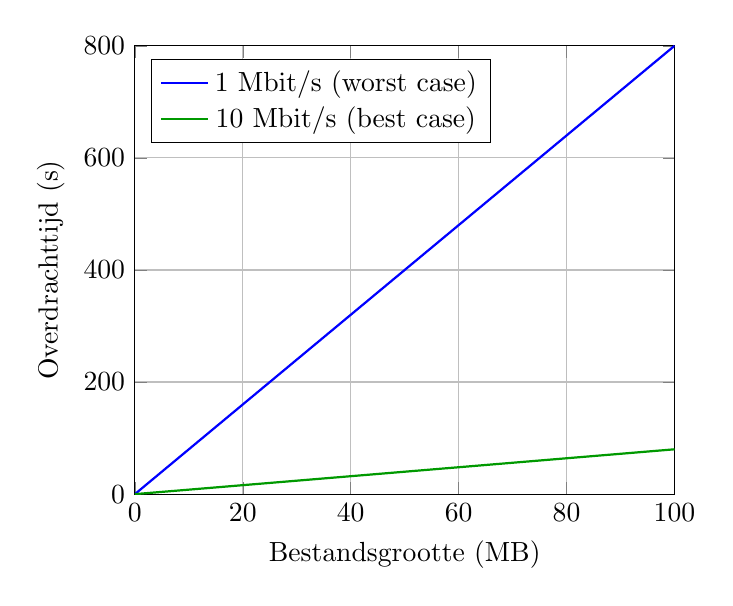
\begin{tikzpicture}
    \begin{axis}[
      xlabel={Bestandsgrootte (MB)},
      ylabel={Overdrachttijd (s)},
      xmin=0, xmax=100,
      ymin=0, ymax=800,
      legend pos=north west,
      grid=major
    ]
    \addplot[blue, thick] coordinates {(0,0)(10,80)(25,200)(50,400)(100,800)};
    \addlegendentry{1 Mbit/s (worst case)}
    \addplot[green!60!black, thick] coordinates {(0,0)(10,8)(25,20)(50,40)(100,80)};
    \addlegendentry{10 Mbit/s (best case)}
    \end{axis}
  \end{tikzpicture}
  \caption{Mock-up: verwachte overdrachttijd in functie van bestandsgrootte bij twee bandbreedtescenario's.}
  \label{fig:mock_bandbreedte}
\end{figure}

Een tweede relevante meting betreft de packet loss in functie van de afstand tussen zender en ontvanger. Op basis van de eigenschappen van straalverbindingen wordt verwacht dat het packet loss percentage laag blijft zolang er een vrije zichtlijn aanwezig is, en sterk toeneemt bij obstructies of bij het overschrijden van de maximale operationele afstand \autocite{MicrowavePtP5G}.

% Mock-up grafiek 2: packet loss vs afstand
\begin{figure}[h]
  \centering
  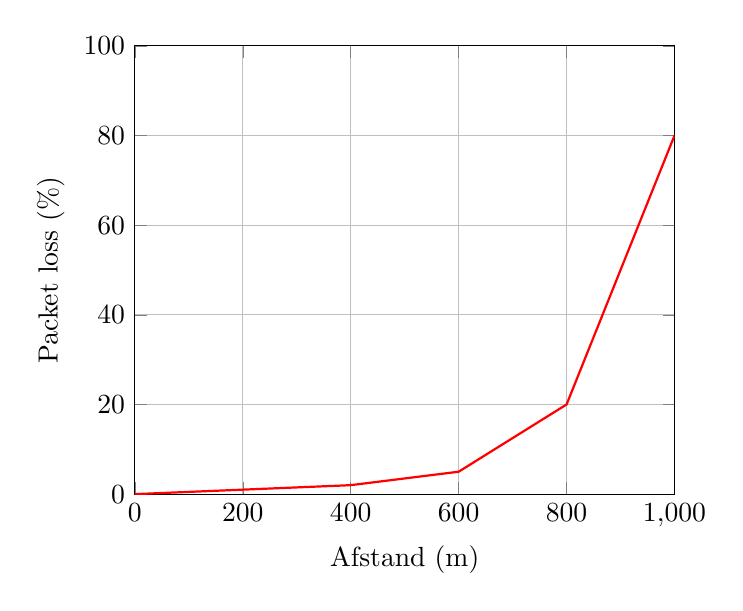
\begin{tikzpicture}
    \begin{axis}[
      xlabel={Afstand (m)},
      ylabel={Packet loss (\%)},
      xmin=0, xmax=1000,
      ymin=0, ymax=100,
      grid=major
    ]
    \addplot[red, thick] coordinates {(0,0)(200,1)(400,2)(600,5)(800,20)(1000,80)};
    \end{axis}
  \end{tikzpicture}
  \caption{Mock-up: verwacht packet loss percentage in functie van de afstand bij een vaste antenneconfiguratie.}
  \label{fig:mock_packetloss}
\end{figure}

\subsection{Meerwaarde voor de doelgroep}

Ongeacht de concrete uitkomst levert dit onderzoek bruikbare informatie op voor IT-professionals en netwerkingenieurs die actief zijn in omgevingen met beperkte connectiviteit. Een werkende proof-of-concept biedt een concreet vertrekpunt voor de uitbouw van robuuste, infrastructuuronafhankelijke bestandstoegangssystemen. Een negatieve uitkomst documenteert de technische grenzen van de huidige aanpak en formuleert aanbevelingen voor alternatieve oplossingsrichtingen. In beide gevallen vult het onderzoek een lacune in de bestaande vakliteratuur, die zich tot op heden niet expliciet heeft gericht op radiogebaseerde toegang tot persoonlijke fileservers.

%%---------- Andere bijlagen --------------------------------------------------
% TODO: Voeg hier eventuele andere bijlagen toe. Bv. als je deze BP voor de
% tweede keer indient, een overzicht van de verbeteringen t.o.v. het origineel.
\chapter{Broncode van de PoC-automatiseringsscripts}%
\label{app:broncode}

Dit hoofdstuk bevat de volledige broncode van de scripts die in
Hoofdstuk~\ref{ch:proof-of-concept} worden besproken en toegelicht. De code wordt hier
ter referentie letterlijk weergegeven; voor de functionele uitleg per script wordt
verwezen naar Sectie~\ref{subsec:scriptoverzicht} en Tabel~\ref{tab:scriptoverzicht-poc}.

\section{Dubbelklikbare startpunten (.bat)}%
\label{sec:app-bat}

\lstinputlisting[style=batchstyle, caption={1-Build.bat}, label={lst:app-1-build}]
  {code/scripts/poc-scripts-windows/1-Build.bat}
\lstinputlisting[style=batchstyle, caption={2-Kies-Scenario.bat}, label={lst:app-2-kies}]
  {code/scripts/poc-scripts-windows/2-Kies-Scenario.bat}
\lstinputlisting[style=batchstyle, caption={3-Voer-Tests-Uit.bat}, label={lst:app-3-tests}]
  {code/scripts/poc-scripts-windows/3-Voer-Tests-Uit.bat}
\lstinputlisting[style=batchstyle, caption={4-Voer-Batchtest-Uit.bat}, label={lst:app-4-batch}]
  {code/scripts/poc-scripts-windows/4-Voer-Batchtest-Uit.bat}

\section{PowerShell-scripts}%
\label{sec:app-ps1}

\lstinputlisting[style=powershellstyle, caption={Build-PoC.ps1}, label={lst:app-build-poc}]
  {code/scripts/poc-scripts-windows/Build-PoC.ps1}
\lstinputlisting[style=powershellstyle, caption={Select-Scenario.ps1}, label={lst:app-select-scenario}]
  {code/scripts/poc-scripts-windows/Select-Scenario.ps1}
\lstinputlisting[style=powershellstyle, caption={Run-Tests.ps1}, label={lst:app-run-tests}]
  {code/scripts/poc-scripts-windows/Run-Tests.ps1}
\lstinputlisting[style=powershellstyle, caption={Run-DistanceTrials.ps1}, label={lst:app-run-distance-trials}]
  {code/scripts/poc-scripts-windows/Run-DistanceTrials.ps1}
\lstinputlisting[style=powershellstyle, caption={Analyze-Trials.ps1}, label={lst:app-analyze-trials}]
  {code/scripts/poc-scripts-windows/Analyze-Trials.ps1}
\lstinputlisting[style=powershellstyle, caption={Modules/PocFunctions.psm1}, label={lst:app-pocfunctions}]
  {code/scripts/poc-scripts-windows/Modules/PocFunctions.psm1}

\section{Cloud-init-manifesten}%
\label{sec:app-cloudinit}

\lstinputlisting[language=yaml, basicstyle=\small\lstmonofont, caption={cloud-init/server-user-data.yaml}, label={lst:app-cloudinit-server}]
  {code/scripts/poc-scripts-windows/cloud-init/server-user-data.yaml}
\lstinputlisting[language=yaml, basicstyle=\small\lstmonofont, caption={cloud-init/link-emulator-user-data.yaml}, label={lst:app-cloudinit-linkemu}]
  {code/scripts/poc-scripts-windows/cloud-init/link-emulator-user-data.yaml}
\lstinputlisting[language=yaml, basicstyle=\small\lstmonofont, caption={cloud-init/client-user-data.yaml}, label={lst:app-cloudinit-client}]
  {code/scripts/poc-scripts-windows/cloud-init/client-user-data.yaml}

%%---------- Backmatter, referentielijst ---------------------------------------

\backmatter{}

\setlength\bibitemsep{2pt} %% Add Some space between the bibliograpy entries
\printbibliography[heading=bibintoc]

\end{document}